% \documentclass[preprint,authoryear,12pt]{elsarticle}
% \documentclass[authoryear,preprint,review,12pt]{elsarticle}
% \documentclass[final,authoryear,1p,times]{elsarticle}
% \documentclass[final,authoryear,3p,times]{elsarticle}
% \documentclass[final,authoryear,3p,times,twocolumn]{elsarticle}
% \documentclass[final,authoryear,5p,times]{elsarticle}
% \documentclass[final,authoryear,5p,times,twocolumn]{elsarticle}

\documentclass[final,authoryear,3p,12pt,times,hidelinks]{elsarticle}

% remove the footnote "preprint submitted to ..."
% \makeatletter
% \def\ps@pprintTitle{%
%    \let\@oddhead\@empty
%    \let\@evenhead\@empty
%    \let\@oddfoot\@empty
%    \let\@evenfoot\@oddfoot
% }
% \makeatother
\makeatletter
\def\ps@pprintTitle{%
     \let\@oddhead\@empty
     \let\@evenhead\@empty
     \def\@oddfoot{\footnotesize\itshape
       \ifx\@journal\@empty
       \else\@journal\fi\hfill\today}%
     \let\@evenfoot\@oddfoot}
\makeatother

%% if you use PostScript figures in your article
%% use the graphics package for simple commands
%% \usepackage{graphics}
%% or use the graphicx package for more complicated commands
\usepackage{graphicx}
%% or use the epsfig package if you prefer to use the old commands
%% \usepackage{epsfig}

%% The amssymb package provides various useful mathematical symbols
% \usepackage{amssymb}
%% The amsthm package provides extended theorem environments
% \usepackage{amsthm}

%% The lineno packages adds line numbers. Start line numbering with
%% \begin{linenumbers}, end it with \end{linenumbers}. Or switch it on
%% for the whole article with \linenumbers after \end{frontmatter}.
%% \usepackage{lineno}


%% Other packages
\usepackage{hyperref}
\usepackage{amsmath}
\usepackage{subfig}
\usepackage{color}
\usepackage{bm}
\usepackage{booktabs}
\usepackage{lscape}

%% natbib.sty is loaded by default. However, natbib options can be
%% provided with \biboptions{...} command. Following options are
%% valid:

%%   round  -  round parentheses are used (default)
%%   square -  square brackets are used   [option]
%%   curly  -  curly braces are used      {option}
%%   angle  -  angle brackets are used    <option>
%%   semicolon  -  multiple citations separated by semi-colon (default)
%%   colon  - same as semicolon, an earlier confusion
%%   comma  -  separated by comma
%%   authoryear - selects author-year citations (default)
%%   numbers-  selects numerical citations
%%   super  -  numerical citations as superscripts
%%   sort   -  sorts multiple citations according to order in ref. list
%%   sort&compress   -  like sort, but also compresses numerical citations
%%   compress - compresses without sorting
%%   longnamesfirst  -  makes first citation full author list
%%
%% \biboptions{longnamesfirst,comma}

% \biboptions{}

\journal{SOCI 40133 Computational Content Analysis}

\begin{document}

\begin{frontmatter}

%% Title, authors and addresses

%% use the tnoteref command within \title for footnotes;
%% use the tnotetext command for the associated footnote;
%% use the fnref command within \author or \address for footnotes;
%% use the fntext command for the associated footnote;
%% use the corref command within \author for corresponding author footnotes;
%% use the cortext command for the associated footnote;
%% use the ead command for the email address,
%% and the form \ead[url] for the home page:
%%
%% \title{Title\tnoteref{label1}}
%% \√tnotetext[label1]{}
%% \author{Name\corref{cor1}\fnref{label2}}
%% \ead{email address}
%% \ead[url]{home page}
%% \fntext[label2]{}
%% \cortext[cor1]{}
%% \address{Address\fnref{label3}}
%% \fntext[label3]{}

\title{State Preferences for Political Agenda and Policy Position Proximity: A Computational Content Analysis Project on the United Nations General Debate Corpus\tnoteref{t1}}
\tnotetext[t1]{This is a final project of the \href{https://github.com/Computational-Content-Analysis-2020/}{SOCI 40133 Computational Content Analysis course instructed by Prof. James Evans at the University of Chicago. Our teaching assistants are Bhargav Srinivasa Desikan and Hyunku Kwon. }}

%% use optional labels to link authors explicitly to addresses:
\author{Luxin Tian}
\author{Heather Chen} 
\address{
  MA Program in Computational Social Science\\
  The University of Chicago
}


\author{}


\begin{abstract}
%% Text of abstract

\end{abstract}

\begin{keyword}
natural language processing \sep international relations \sep united nations

\end{keyword}

\end{frontmatter}

% \linenumbers




%% main text
\section{Introduction}

There has been a growing interest in quantitatively measuring preferences of political agents in the field of political science. While qualitative approaches through case studies or historical analyses have been conanical in this field for centuries, quantitative measurement provides a more comprehensive and systemmatic framework in which the characteristics and dynamics revealed by actions of political agents can be identified, tracked, and analyzed. In the digital age, actions of political agents, such as parties, governments, and international organizations, can be traced in miscellaneous forms, and the development of data mining tehniques and the computation capability unlocks new possibilities for researchers to reveal preferences of political agents through documented actions. 

In this project, we perform an exploratory computational content analysis on the United Nations General Debate Corpus (UNGDC) to extract insights into state political preferences and positions from documented speeches. The UNGDC, which has been introduced and maintained by \cite{baturo2017understanding} and \cite{DVN/0TJX8Y_2017}, currently consists of 8093 statements made by state governments or heads of state at the annual General Debate of the United Nations General Assembly from 1970 to 2018. All the statements have been processed and converted to text files and organized by countries and sessions. Incorporating several prevailing techniques in Natual Language Processing, we make inference about international politics on two dimensions. First, we investigate the preferences for political agenda of international political agents, or, more specifically, the variation and dynamics of states' emphsis on certain topics of their concerns. Second, we extract position information of each state from the statements and quantify the dynamic similarities between sates in a political position space. As we will show in section \ref{sec:Results}, benefited from the inclusiveness and competitiveness of the UNGDC corpus, we are able to examine several aspects of contemporary international politics from a comprehensive perspective. Most of our data processing and computational analysis work is performed in Python. 

As is argued by \cite{baturo2017understanding}, the General Debate statements data has several favorable properties for comparative political analysis. For one thing, the lack of military allies for some states and the limited number of issues that are voted on in international conferences make such indicators incomplete and biased for measuring political preferences. In contrast, the General Debate provides all the member states of the United Nations an equal opportunity to address their positions on issues of their concerns to the international society. For another thing, due to loose institutional connection to the decision-making process, the General Debate statements are less constrained by external pressures from other states than voting actions are, so that the contents would reflect more about the real interests and positions of states. These features make it more reliabile and complete to use the UNGDC for revealing and measuring political preferences than using military alliances or voting records as proxy indicators. 

In light of the advantages of the UNGDC, we assume through the whole analysis that the UNGDC is complete and unbiased for revealing political preferences and ideologies in a way that it contains semantically meaningful sentences that address political positions and concerns. Obviously, this assumption may not be completely true. First, as we will show, the lengths for statements become more and more limited as the number of participating states increases over year. As a result, since states may have priorities on elaborating certain issues over others, the compressed content may not represent the complete ideologies on all issues, and the distribution of emphasis on each topic can also vary across states and sessions. Second, the states may still face external pressures from other states when delivering the statements even though the opportunity is institutionally equal for all member states. This can result that the semantic meaning of one state's expressions are not independent but correlated to other states. If it is the case, the robustness and reliability of our inference would be qualified. However, we argue that the UNGDC still outperforms many other data source for empirical analysis of state political preferences for the reasons mentioned above, and we will address potential drawbacks and our reflections of this research in sections \ref{sec:Reflections and Extensions} of this report. 

In section \ref{sec:Methods}, we review the computational methods that we employed in this project and evaluate the fitness of each method to our research question. For some of the methods, we also introduce our implementation of the algorithms and evaluate the computational performance of the program. In section \ref{sec:Results}, we present our findings and relate the some of the results to historical events and contexts. Finally, in section \ref{sec:Reflections and Extensions}, we assess the reliability and validity of our analysis, clarify potential drawbacks, and propose future extensions of our research. 

\section{Data}

The United Nations General Debate Corpus (UNGDC) has been published and maintained by \cite{DVN/0TJX8Y_2017}. The latest update of the corpus consists of 8093 statements delivered by 200 states on the annual sessions of the Univeted Nations General Assembly from 1970 to 2018. The comprehensive historical miscellaneous data for each session, based on which this corpus was built, is published on the website of the General Assembly of the United Nations in the forms of full-text \texttt{.pdf} documents, audio, video, and summary text in all the six official working languages. The UNGDC incorporates all the English version documents that record the statements made by state leaders or government representatives. Each document has been converted to a \texttt{.txt} file and categorized and labelled by a alpha-3 country code (ISO 3166), the session number, and the year. 

\begin{table}
    \centering
    \caption{Preview of the UNGDC corpus}
    \label{data preview}
    \resizebox{\textwidth}{!}{
        \begin{tabular}{lllll}
        \toprule
                filename & country\_code & session &  year &                                               text \\
        \midrule
        ALB\_25\_1970.txt &          ALB &      25 &  1970 &  33: May I first convey to our President the co... \\
        ARG\_25\_1970.txt &          ARG &      25 &  1970 &  177.\textbackslash t : It is a fortunate coincidence that pr... \\
        AUS\_25\_1970.txt &          AUS &      25 &  1970 &  100.\textbackslash t  It is a pleasure for me to extend to y... \\
        AUT\_25\_1970.txt &          AUT &      25 &  1970 &  155.\textbackslash t  May I begin by expressing to Ambassado... \\
        BEL\_25\_1970.txt &          BEL &      25 &  1970 &  176. No doubt each of us, before coming up to ... \\
        BLR\_25\_1970.txt &          BLR &      25 &  1970 &  \textbackslash n71.\textbackslash t. We are today mourning the untimely de... \\
        BOL\_25\_1970.txt &          BOL &      25 &  1970 &  135.\textbackslash t  I wish to congratulate the President o... \\
        BRA\_25\_1970.txt &          BRA &      25 &  1970 &  1.\textbackslash tMr. President, I should like, first of all... \\
        CAN\_25\_1970.txt &          CAN &      25 &  1970 &  \textbackslash nThe General Assembly is fortunate indeed to ... \\
        CMR\_25\_1970.txt &          CMR &      25 &  1970 &  : A year ago I came here as the Acting Preside... \\
        \bottomrule
        \end{tabular}
    }
    
    \end{table}

The number of states that deliever the statements on each session varies across years, but overall it has been gradually increasing from 71 in 1970 to 200 in 2018. We identify these changes and include a table showing the change of participating states for each year in the appendix. 

We preprocess the corpus by tokenizing the words in each document into lists of tokens, normalizing the tokens, removing digits, punctuations, non-latin characters, and English stop words, and then lemmatizing. For some of the modeling procedures that we introduce in the next section, we also perform stemming on the normalized tokens, which reduces the tokens into their base forms. For tokenization and normalization, we take advantage of the helper functions from the \href{https://github.com/Computational-Content-Analysis-2020/lucem_illud_2020/}{\texttt{lucem\_illud\_2020}} package. For stemming we use the \texttt{PorterStemmer} implemented by the \href{https://www.nltk.org/}{\texttt{NLTK}} package. 

After tokenizing, we count the number of tokens in each document and calculate the mean token count per statement. As is shown by figure \ref{fig:number of states and mean token count}, with the number of participating states increased over years, the mean token count steadily reduced almost in half, indicating the speakers face more and more rigorous time limitation when delivering the statement speech. However, the mean token count still remains as high as around 2,000. 

\begin{figure}[ht!]
  \begin{center}
    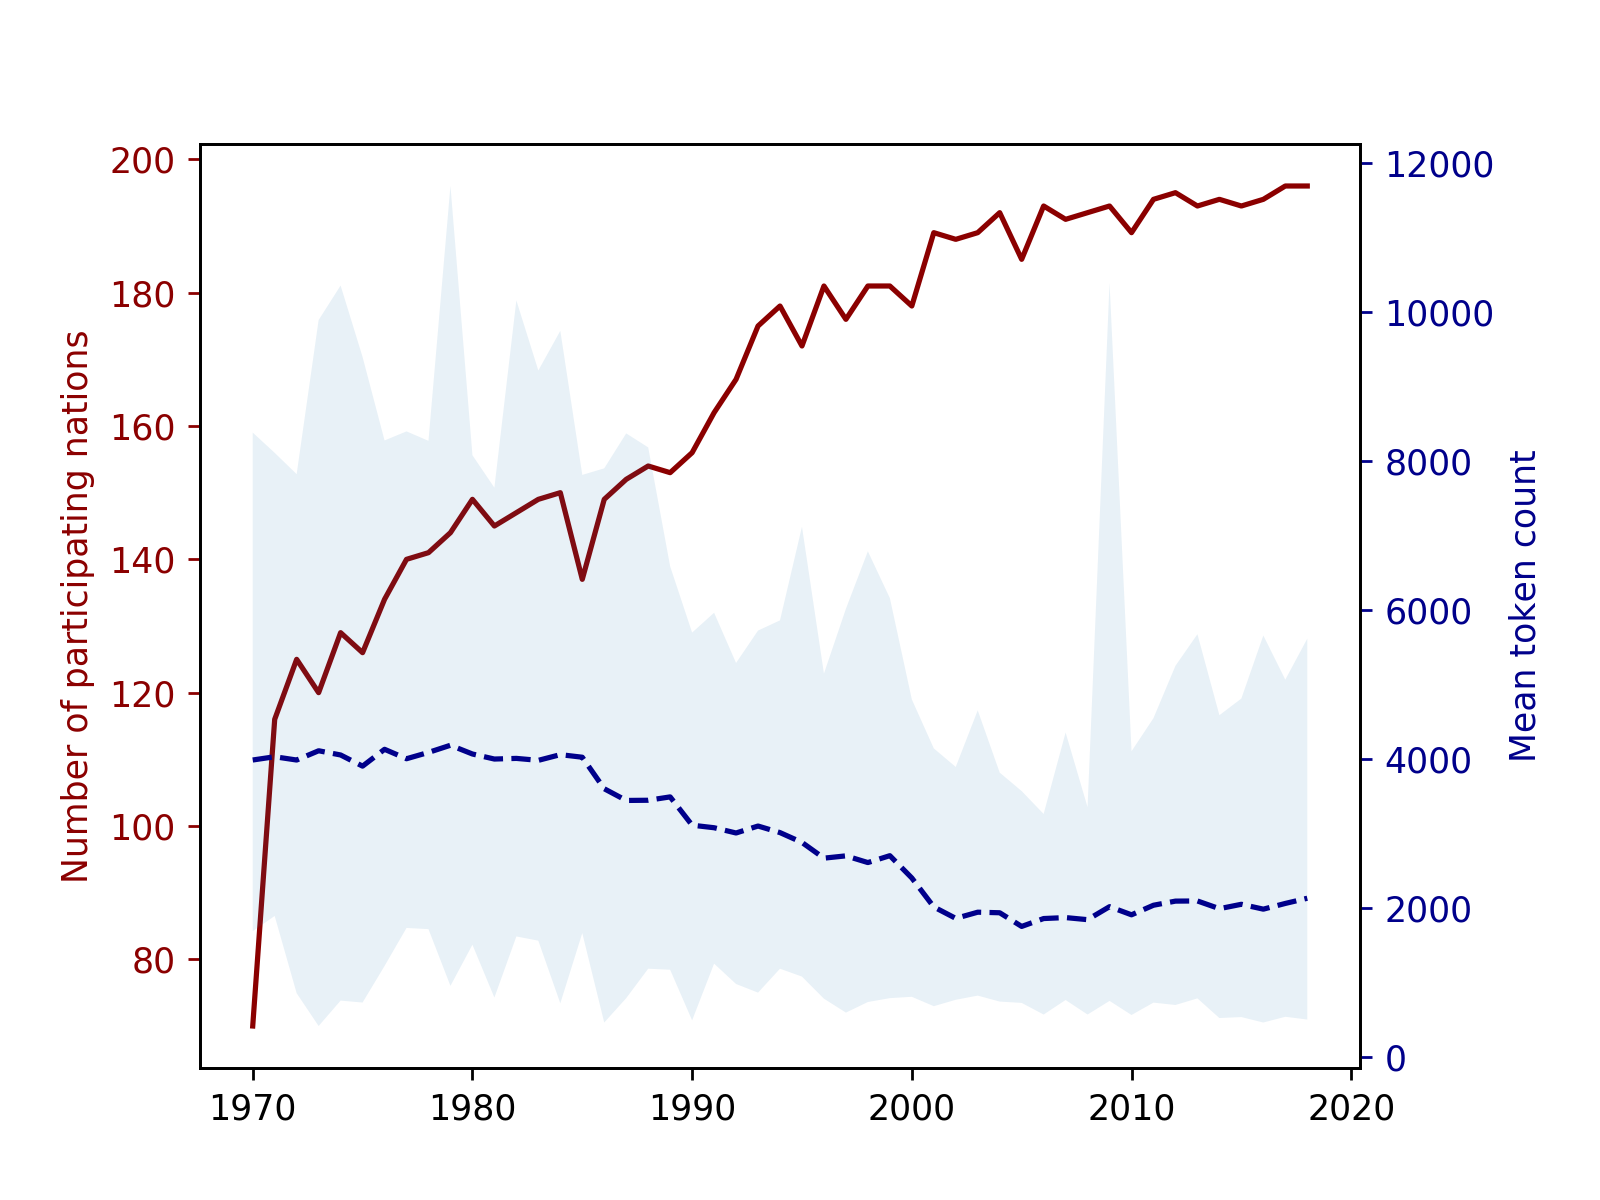
\includegraphics[width=0.7\textwidth]{graphs/number_of_states_and_mean_token_count.png}
    \caption{Number of Participating Nations and Mean Token Count per Statement (1970-2018)}
    \label{fig:number of states and mean token count}
  \end{center}
\end{figure}

We arrange this corpus and organize it into the following format. For each document, we label it with a three-letter country code, an integar indicating the session, and another integar indicating the year. We save the results of tokenization and normalization into two separate columns for future use. Note that in the original UNGDC corpus one text document \texttt{URY\_40\_1985.txt} was mistakenly named as \texttt{URY\_49\_1985.txt}. We have corrected it by hand. 

% \begin{table}
% insert the dataframe.   
% \end{table}

\section{Methods and Implementations}
\label{sec:Methods}

The UNGDC corpus contains rich information about national political positions on a wide range of issues and topics. In this section, we briefly review the methods we employ to gain insights into the social mechanism underlying the data generating process of the text. First, we examine word frequency. On this basis, we identify the most common words conditional on their functions as parts of speech to reveal the most significant object being discussed in the recent decades. We also try to directly quantify the proximity of state positions by extracting the principle components of the word frequency vectors as well as performing a K-means clustering on the vector space. Second, we embed the tokens onto a semantic space using the techniques named Word2Vec and Doc2Vec, based on which we investigate position proximity between states from a semantic perspective. Third, we turn to topic modeling and employ the Latent Dirichlet Allocation model to figure out the topics that the states concerned over years. Finally, we also construct international networks based on mutual information revealed by topic modeling to measure position proximity in terms of topics of common interests. 

\subsection{Word Frequency: Term Frequency - Inverse Document Frequency (TF-IDF)}
\label{sub:TF-IDF}
The Term Frequency - Inverse Document Frequency (TF-IDF) measures the frequency of a word in a document normalized by the importance of docuemnts in the whole corpus. Intuitively, it reduce the weights of the frequency of the words in a document that occur very frequently in the whole corpus. 
% If some word is highly frequent in one document, but very rare in the whole corpus, we can infer that this word is significant to this specific document. On the contrary, if some word is not only frequent in one document but also frequent in the whole corpus, it is reasonable to regard it as a common word and thus not significant for this specific document. 
To characterize this normalized measurement of word frequency, for each token $t$ in a document $d$, the formula of TF-IDF is given by: 
\begin{equation}
  \begin{aligned}
    \text{TF-IDF}(t, d)
    &= \text{Term Frequency (TF)} \times \text{Inverse Document Frequency (IDF)} \\
    &= \frac{\text{count of }t \text{ in } d}{\text{number of tokens in }d} \times \ln(\frac{\mathrm{\text{count of }t\text{ in corpus}}+1}{N})
  \end{aligned}
\end{equation}

We use \texttt{sklearn.feature\_extraction.text.tfidfvectorizer} to extract the word frequency features for each token in each document of our corpus, which gives a document-token TF-IDF matrix. Each row of this matrix can be viewed as a feature vector characterizing each document in terms of the relative significance of its tokens. 

We assume that the content of a statement can be represented by its TF-IDF vector, which is expected to contain multidimensional information about the topics that the state concerns and their position and ideology on the topics. Even though the topics are not directly observable nor identifiable by the TF-IDF vector, we can compare any two documents by comparing the two TF-IDF vectors to infer the similarity of the content in the normalized word frequency space. 

Based on the TF-IDF matrix, we perform two analyses. First, we reduce the dimensionality of the vectors using Principle Component Analysis (PCA) to unidimensional scalars. We expect this to abstractly represent the content of the statements in the TF-IDF space, which is equivalent to project multi-dimensional state preference to one single visible dimension. Then, we take several countries as examples and visualize the the revelation of several countries' preference over years. Second, we perform K-means clustering using the TF-IDF vectors associated with each document. We review and evaluate the K-means Clustering method in section \ref{subsec:K-means Clustering}

\subsection{Part-of-Speech Tagging}
\label{subsec:Part of Speech}
Part-of-Speech (POS) Tagging is to parse a document of natural language and tag the grammatic role of each token in a sentence. Since it depends on the grammatic context to disambiguate the word category, we use the \texttt{SpaCy}'s implementation of POS tagging to parse our documents using the original text without lemmatizating or normalizing. Note that one of the most frequent words "coorperation" is commonly written as "co-orperation" in our corpus, and the POS tagger fails to identify it as a single word, we have corrected it to "coorperation" by hand before performing POS tagging. Conditional on word categories, we can count token frequency and figure out the most frequently-used word of certain grammatic category in our corpus, which can relfect the general topics and the main content of this international politics corpus. 

\subsection{Word Embeddings and Semantic Space: Word2Vec and Doc2Vec}
\label{subsec:Word Embeddings}
Word embedding is a language modeling technique that maps words to vectors in a semantic space, of which \texttt{Word2Vec} and \texttt{Doc2Vec} are two computational implementations. In the resulting vector representations of words, similar words with similar semantic meanings turn out to be close to each other \citep{mikolov2013efficient}. While \texttt{Word2Vec} embeds each token into a semantic space and represents tokens as numeric feature vectors, \texttt{Doc2Vec} enables us to label each documents as sets of tokens and create numeric representations of documents in the same sematic space where the words are embedded. As a result, the word vectors can be thought as representations of the semantic meaning of each single word, and the document vectors represents the meaning of each document. 

In our ananlysis, we train a \texttt{Doc2Vec} model with our corpus using the implementation by \texttt{gensim.models.doc2vec}. Based on the resulting semantic space, we can quantify the proximity of any two states' position by calculating the cosine similarity of their document vectors. We can also assign hirerachical labels to the documents to integrate the features of all the documents of one state over years into a single vector. On this basis, we can project the states onto certain dimensions we define to answer our research question, for example, the Cold War dimension specified by the differences between the vectors of the NATO and the WTO states as well as `capitalism' and `socialism'. Furthermore, we perform K-means clustering using the documentation vectors to identify state blocs in terms of their overall standpoints of the Cold War extensive issues. 

To verify that our corpus is complete and rich enough to construct a semantic space with meaningful results, we pretrain a \texttt{Word2Vec} model and experiment with several vector operations. We can find the most semantically similar words to a word. We can also perform vector operations to find the most matching word to an equation such as $\text{king} - \text{queen} = \text{man} - \text{women}$, which is one of the examples presented by \cite{mikolov2013efficient}. We have many interesting results (shown in Table \ref{tab:word2vec similar words} and \ref{tab:word2vec operations}). 

\begin{table}[ht!]
  \centering
  \caption{Examples of finding the most similar words}
  \begin{tabular}{c c} 
  \hline
  target word & similar words \\
  \hline 
  economic & socioeconomic, macroeconomic, economy, economies \\

  political & institutional, geopolitical, politico, civic \\

  socialism & communism, revolution, militarism, fascism \\
  \hline
  \end{tabular}
  \label{tab:word2vec similar words}
\end{table}

\begin{table}[!ht]
  \centering
  \caption{Examples of vector operation in the semantic space}
  \begin{tabular}{c c c c c c c} 
  \hline
  token$1$ & $-$ & token$2$ & $=$ & token$3$ & $-$ & token$4$\\
  \hline
  american & - & america & = & korean & - & korea \\ 
  
  islamabad & - & pakistan & = & bangkok & - & thailand \\
  
  oppose & - & support & = & reject & - & welcome \\
  \hline
 \end{tabular}
 \label{tab:word2vec operations}
\end{table}

\begin{figure}[ht!]
  \begin{center}
    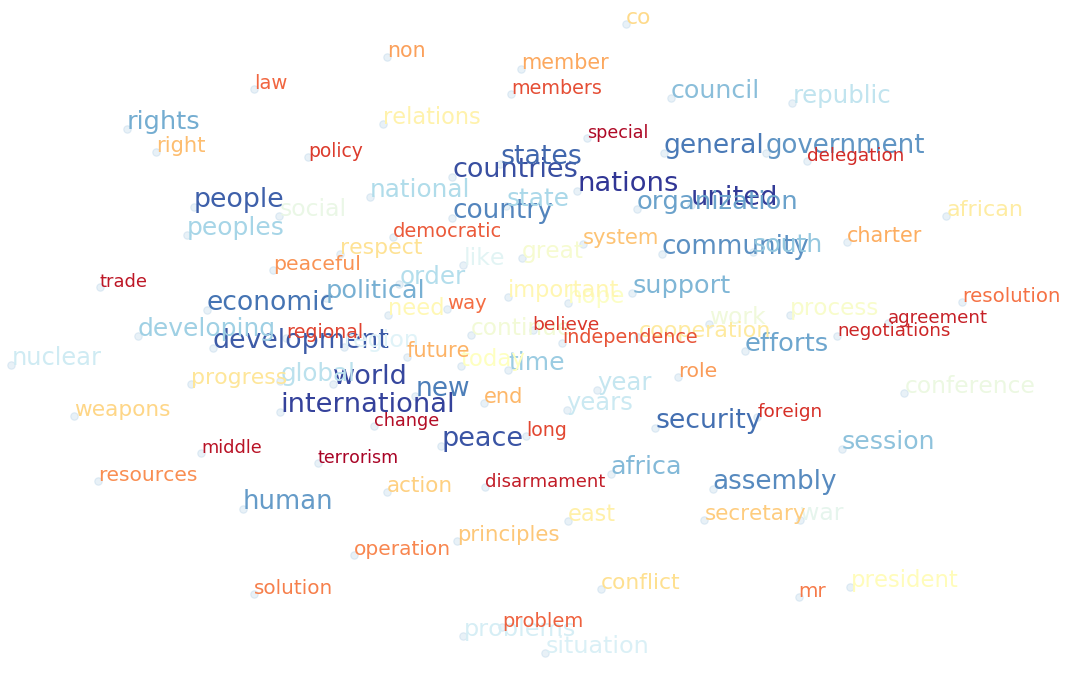
\includegraphics[width=0.8\textwidth]{graphs/word2vec_semantic_space.png}
    \caption{Top 100 words in the Word2Vec semantic space (dimension-reduced)}
    \label{fig:word2vec space}
  \end{center}
\end{figure}

We can also visualize the semantic space where the words or documents are embedded. Since the vectors are high dimensional, we perform dimension reduction using the Principle Component Analysis (PCA) implemented by \texttt{sklearn.decomposition.PCA} and the t-distributed Stochastic Neighbor Embedding (tSNE) implemented by \texttt{sklearn.manifold.TSNE}. While PCA is a technique for linear dimensionality reduction, tSNE is a specific tool to visualize high-dimensional data \citep{maaten2008visualizing}. Since PCA is computationally efficient, we use PCA decomposite the vectors in the semantic space to 100 dimensions prior to using tSNE to project the vectors onto a two-dimensional space. Note that \texttt{gensim.models.word2vec.Word2Vec} sorts the vocabulary by descending frequency by default, we selected the first 100 most frequent words in the corpus and visualize their positions in the semantic space in Figure \ref{fig:word2vec space}. We can observe, for example, `state', `states', `country', `countries`, `nations', and `national' are located close to each other. Note that colors are proportional to the font size from blue to red, which reflects the frequency of a word in the whole corpus. 

Similar results can be found in the \texttt{Doc2Vec} semantic space. For example, we find that the most similar states in terms of text content to `USA' are `GBR', `CAN', `ISR', `AUS', `NOR', `NZL', `NLD', etc, which are consistent to the reality that the UK, Canada, Norway, and the Netherlands are member states of the North Atlantic Treaty Organization (NATO), and Israel, Australia, and New Zealand are designated by the US government as Major non-NATO Allies (MNNA). 

Such evidence shows the UNGDC corpus contains information that is complete and rich enough to construct a meaningful semantic space, from which we can make inference about the relations between countries in terms of political positions and opinions on issues and the dynamics over years. 

\subsubsection{Cosine Similarity}
\label{suc:network Cosine}
With the vectors representing the documents in the semantic space, we can evaluate the similarity between any two vectors by calculating the cosine similarity. The formula is given by: 
$$ \cos{(\bm{a}, \bm{b})} = \frac{\bm{a} \cdot \bm{b}}{\left\|\bm{a} \right\| \cdot \left\|\bm{b} \right\| } \in [0, 1]$$
, where $\bm{a}$ and $\bm{b}$ are any two vectors in the corpus. The higher the consine similarity, the more similar the two vectors are in terms of semantic meanings. 

We perform two analysis. First, we examine the similarities between states in the over years by calculating pairwise cosine similarities of the state vectors. We visualize the result in a heatmap. To alleviate noisy variations across years, we also show the average cosine similarities between states every five years to detect the most significant dispute and consensus. We will give the standard deviation of the cosine similarities at the end of the analysis, which indicates the variation of international relationship in terms of policy proximity over years. 

Second, we investigate the dynamics of international attention paid on specific policy areas by calculating the consine similarities between the year vectors and the vectors representing the keywords of several policy topics. For the topics characterized by more than one token, we use the mean of multiple vectors to construct the basis vector. We can also observe the attention to such topics paid by specific states and evaluate to what extent these states are leading the international discussion of the policy issues in the United Nations. 

\subsection{K-means Clustering}
\label{subsec:K-means Clustering}
K-means Clustering is an unsupervised learning method that partitions feature vectors into $k$ clusters aiming at minimizing the sum of squared distance from each observation to the centroid with each cluster. We fit the model implemented by \texttt{sklearn.cluster.KMeans} using both the TF-IDF vectors and the \texttt{Doc2Vect} vectors as the features. 

Fitting with the TF-IDF vectors, we cluster the single documents featured by distributions of normalized word frequency. We assume documents with similar TF-IDF vectors are likely to elaborate state positions about similar political agenda. On this basis, we can reveal the topics within each cluster by querying the most distinguishing words, in terms of TF-IDF scores, of the cluster centroids. Although this analysis reveals very limited information about the preference for political agenda of any specific state, it can help us with an overall impression about what the topics are discussed in the UN General debate in the past half century. 

Using the state vectors in the \texttt{Doc2Vec} semantic space, we are to identify state blocs in the semantic space, respectively. Since each vector represent the content of all the satetments of one state as a whole, partitioning such vectors can reveal the state blocs in terms of position proximity. We also experiment by fitting the model using a subset of the corpus during the Cold War period, trying to identify state blocs in the Cold War years. 

To tune the parameter $k$, the number of clusters, we use \texttt{Silhouette} coefficient as a metric. The Silhouette is a measure of the extent to which an observation is similar to its own cluster compared to it is to other clusters. The higher the Silhouette is, the more coherent and less separative the observations within each clusters are. For our clustering model using TF-IDF vectors, the optimal $k$ value is 36 (shown in Figure \ref{fig:kmeans tunning tfidf}). For the model using Doc2Vec vectors, the optimal $k$ value is 5 (shown in Figure \ref{fig:kmeans tunning doc2vec}). 

\begin{figure}[ht!]
  \centering
  \subfloat[Silhouette Coefficient for $k=5$]{{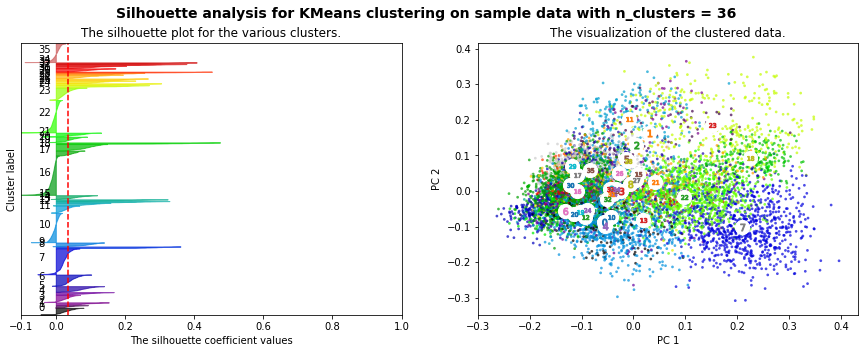
\includegraphics[width=0.9\textwidth]{graphs/k_means_tuning_tfidf.png} }}
  \qquad
  \subfloat[Silhouette Coefficients for different $k$ values]{{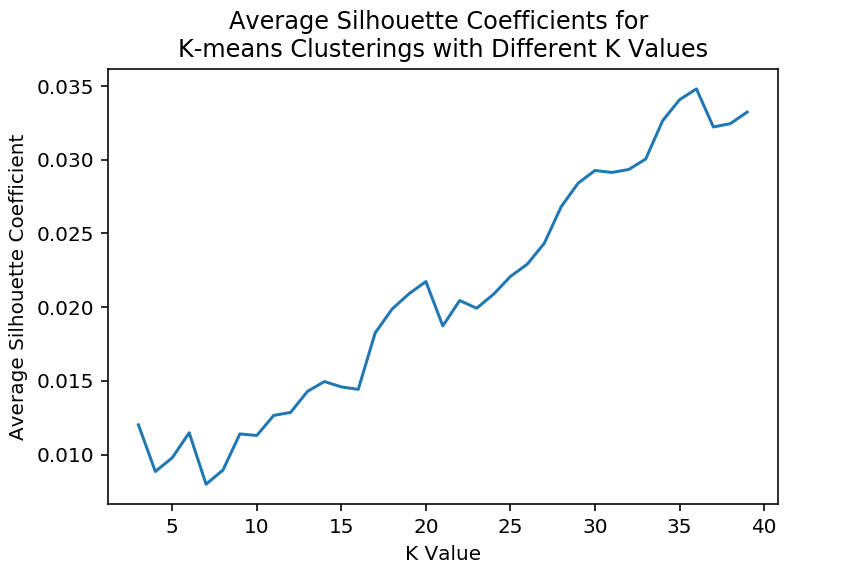
\includegraphics[width=0.5\textwidth]{graphs/compare_k_means_tuning_tfidf.png} }}
  \caption{Parameter tuning for K-means Clustering using Doc2Vec vectors}
  \label{fig:kmeans tunning tfidf}
\end{figure}

\begin{figure}[ht!]
  \centering
  \subfloat[Silhouette Coefficient for $k=5$]{{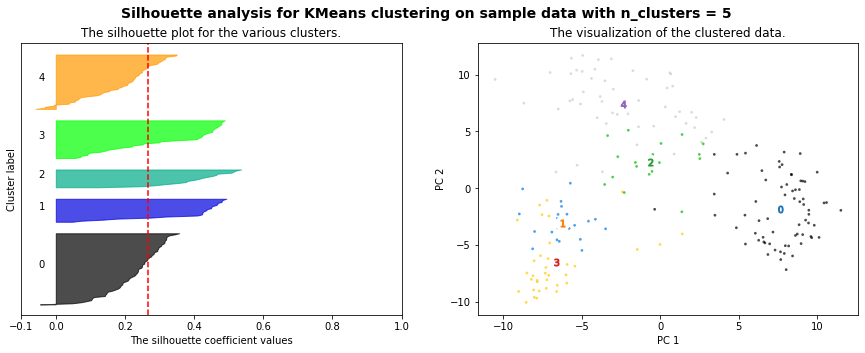
\includegraphics[width=0.9\textwidth]{graphs/k_means_tuning_doc2vec.png} }}
  \qquad
  \subfloat[Silhouette Coefficients for different $k$ values]{{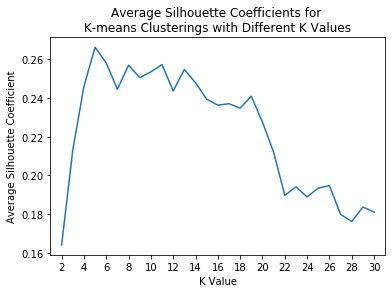
\includegraphics[width=0.5\textwidth]{graphs/compare_k_means_tuning_doc2vec.png} }}
  \caption{Parameter tuning for K-means Clustering using Doc2Vec vectors}
  \label{fig:kmeans tunning doc2vec}
\end{figure}

\subsection{Topic Modeling}
\label{subsec:Topic Modeling}
Topic Modeling is a method used for extracting abstract “topics” in a set of given documents. In topic modeling, a document is represented by a distribution of topics, while a specific topic is represented by a probability distribution over a set of words. Words that are assigned with higher probability can better reflect the main ideas in this topic \citep{griffiths2007topics}. In this paper, we use two different methods, Latent Dirichlet Allocation model and Dynamic Topic Modeling, to address this issue from different perspectives. 

\subsubsection{Latent Dirichlet Allocation (LDA) Model}
\label{subsec:LDA}
Topics are important features that we focus on in this paper. By looking at the distribution of probabilities of a certain speech on different topics, we may discover what kind of issues the country that proposed this speech is putting spotlights on. This information is then utilized to construct network analysis in the following section. Furthermore, generalized from a larger perspective, we may come to conclude the most heated topics in United Nations General Debate, or in the worldwide, throughout the 49 years.

Latent Dirichlet Allocation (LDA) model is one of the most widely used techniques for topic modeling. In this model, topics are presented as latent variables that cannot be observed. At the first two steps of LDA model, $\theta_i$, the topic distribution for the document $i$ in the corpus and $\phi_k$, the word distribution for the topic $k$ are characterized by two separate Dirichlet distributions at given Dirichlet prior parameters $\alpha$ and $\beta$. Then it supposes that $z_{i,j}$, the topic for the $j$-th word in document $i$ can be expressed by a multinomial distribution of $\theta_i$. Given the conditions above, a specific word at position $j$ at a specific document $i$ can therefore be represented by a multinomial distribution with the topics as an embedded layer \citep{blei2003latent}.  

The first step of LDA topic modeling in this paper is choosing the optimal parameters to obtain the most meaningful and interpretable topic results. Before conducting LDA analysis, we restrict the vocabulary using TF-IDF measures to ignore words that appear too often in the corpus. In the TF-IDF measure, we also set up a tokenizer to stem words which length are less than 4 letters. In order to acquire the optimal results of topics, we choose different levels of \texttt{max\_df} \footnote{A float between 0 and 1, used to indicate a proportion of documents, and words that has term frequency higher than that value is ignored. } parameter to compare the performance of LDA model under different TF-IDF filtering standards. 

The number of topics is another factor that we take into consideration when selecting the best LDA model. A satisfying topic number can capture the most information in the corpus and produces the most meaningful topic results. Given the two parameters of interest stated above, we use the UMass coherence score to evaluate the performance of LDA model. UMass is an intrinsic measurement of topic coherence, which captures how well the topic model `explains' our corpus of interest. The less the UMass coherence score is, the better interpretability of the model. Figure \ref{fig:umass coherence num topics} below illustrates the coherence score under different \texttt{max\_df} level against different number of topics.

\begin{figure}[ht!]
  \begin{center}
    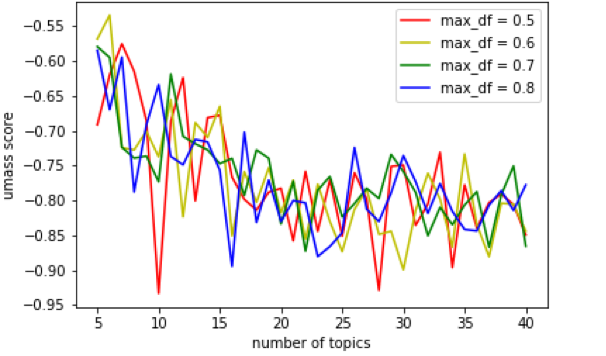
\includegraphics[width=0.8\textwidth]{graphs/umass_coherence_num_topics.png}
    \caption{UMass coherence scores for different number of topics}
    \label{fig:umass coherence num topics}
  \end{center}
\end{figure}

As we can see, the LDA model has the best interpretability when setting \texttt{max\_df = 0.5} and choosing the number of topics equal to 10 or 28. After printing out the top feature words in each topic under these two topic numbers, we use \texttt{num\_topic = 28} for further analysis as it captures more information. 

Using LDA topic modeling alone, we present the top 10 words with the highest probability in each topic. For some of these topics, we make a speculation of what are they mainly talking about. Besides, we use a Python package called \texttt{pyLDAvis} to visualize our topic model generated above. Other applications of LDA model are stated in Section \ref{sec:Network Contraction}.


\subsubsection{Dynamic Topic Modeling}
\label{subsec:DTM}
[Introduce DTM...]



\subsection{Network Contraction: Mutual Information}
\label{sec:Network Contraction}
Semantic networks are representations of semantic relationships between concepts of interest in the corpus. A semantic network has two key elements: nodes that represent concepts, and edges that can be directed or undirected, which represent the semantic relationship between linked concepts. 

Based on the argument of \cite{gurciullo2017topology}, we can regard topics extracted from LDA model as having semantic values. Countries whose speeches cover similar topics show their overlying interest in similar political issues. In the last section, we use LDA model to construct a vector that constitutes of topic probabilities of the 28 topics for each country in every year. Therefore, in each of these 49 years, if we view each country (represented by a topic probability vector) as an individual semantic entity, we can build a semantic network based on the similarity of their topics of interest. The similarity is measured in normalized mutual information score, which will be introduced in detail in the following section. 

In this paper, we construct 49 separated semantic networks. We first investigate several statistics that reveals the overall structure of the network such as density, average shortest length path, and diameter. Further on, by looking at the individual nodes of the graph, we can make inquiries about which countries are in the center of this network, which countries are on the border, and which countries are usually linked with one another. In the end of our network analysis, we go on to explore how a country’s `position' in the network evolves over years through different measurements of centrality. 

\subsection{Mutual Information}
\label{sec:Mutual Information}
In the LDA model, for each country that has given a speech in each year, we obtain a vector of topic prevalence that describes the probability that the speech might load on each of the 28 topics. These can be intercepted as probability distributions, whose similarities between one another can be measured using the mutual information coefficient. 

Mutual information captures the mutual dependence of two random variables. Since vectors here can be interpreted as discrete probability distributions, we might write the mutual information measurement as the following: 
$$I_{X;Y}=\sum_{y \in Y} \sum_{x \in X} p_{X,Y} (x,y) \ln{\frac{p_{X,Y} (x,y)}{p_X (x) p_Y (y)}}
$$
, where $X$ and $Y$ is the random variable of interest, $p_{X,Y} (x,y)$ is the joint probability density function of $X$ and $Y$, and $p_X (x)$ and $p_Y (y)$ are the marginal probability density functions of $X$ and $Y$, respectively. 

The value of mutual information indicates how much the two random variables share information. In this case, a low mutual information score that close to zero denotes the two countries are focusing on different topics, while a relatively high mutual information score can be viewed as the two countries are paying attention to similar topics in that year. For the purpose of comparison, we normalize the mutual information score computed above to a float between 0 and 1. The normalized mutual information score is what we used to construct edges in the semantic network. 

\subsubsection{Construct Network using Mutual Information}
\label{suc:network MI}
After obtaining the normalized mutual information score between any two countries that have delivered a speech in a given year, we establish a semantic network whose nodes are countries. This network is completely linked at the first place, where the weight of the edge between two nodes is defined by the normalized mutual information score. 

For the simplicity and interpretability of the network, we remove edges whose weights are below the median weight of the network. This step ensures that our networks only retain semantic relationships between countries above a certain threshold. Also, for years between 1970 and 1991, we assign different colors to nodes that represent NATO countries and WTO countries. An example of the network is shown in Figure \ref{fig:network MI 1972}. 

\begin{figure}[ht!]
  \begin{center}
    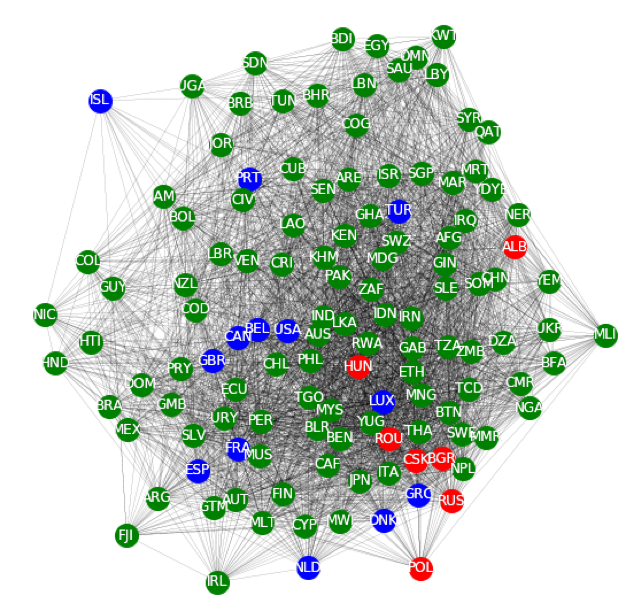
\includegraphics[width=0.8\textwidth]{graphs/1972_mutual_info_network.png}
    \caption{State Network of Mutual Information (1972; NATO states in blue and WTO states in red)}
    \label{fig:network MI 1972}
  \end{center}
\end{figure}

\section{Results}
\label{sec:Results}
Employing the methods introduced in the previous section, we try to answer two research questions. First, we examine what topics states are concerned about and how the attentions paid to specific issues evolve over years. Second, we examine the patterns in which the states are related to each other in terms of topics of common concerns, political positions, and policy preferences, and the dynamics of the relationship. 

\subsection{State Preferences for Political Agenda}
The most frequent words in this corpus hints us with an overal impression about the general topics being discussed on the UNGA in the past half century. While, peace and development are the theme of the era, economic development, nuclear security, human rights, etc, are the common issues concerned by the international society. 

\begin{figure}[ht!]
  \centering
  \subfloat[The most frequent nouns]{{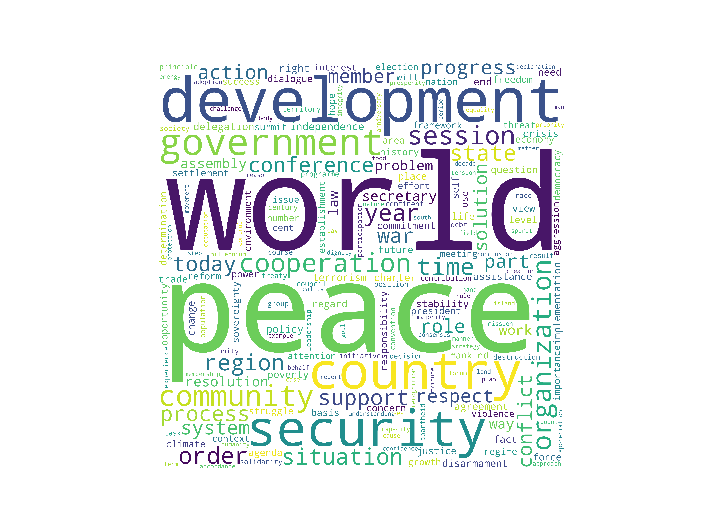
\includegraphics[trim=75 0 75 0, width=0.475\textwidth]{graphs/freq_noun.png} }}
  \quad
  \subfloat[The most frequent adjectives]{{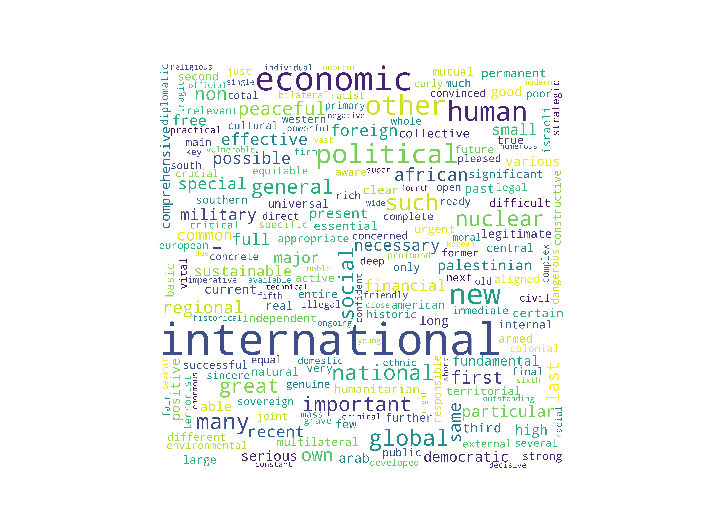
\includegraphics[trim=75 0 75 0, width=0.475\textwidth]{graphs/freq_adjs.png} }}
  \caption{The most frequent words in the corpus}
  \label{fig:freq words}
\end{figure}

We try to gain further insights into agenda topics by performing K-means clustering on the TF-IDF matrix. We query the most distinguishing patterns of each cluster centroids, which is, equivalently, the words with the highest TF-IDF scores associated with each cluster centroid. The clustering result is shown in Table\ref{tab:kmeans tfidf centroids1}, \ref{tab:kmeans tfidf centroids2}, \ref{tab:kmeans tfidf centroids3}, and \ref{tab:kmeans tfidf centroids4}. Unfortunately, the result shows no coherent topic within each cluster, but we still pick up some meaningful topics from the results: terrorism, nuclear weapons, disarmament, climate change, drug abuse, poverty alleviation, etc. Such results help us as evidence to validate the result of our topic subsequent modeling analysis. However, the clusters are less meaningful in revealing agenda topics due to transparent fallacy, which we discuss in Section \ref{sec:Reflections and Extensions}. 

[Topic Modeling]

[Topic Modeling]

[Topic Modeling]

[Topic Modeling]

We turn to the analysis based on the Doc2Vec semantic space. Recalling that we have labelled the documents with year and country code, we can examine the consine similarity of the year vectors and other vectors representing specific issues. This allows us to reveal the dynamics of attentions paid on the issues over years. We choose the issues in Table \ref{tab:attention dynamics choose issues} and select the corresponding key words to construct the basis vectors. Note that our result is robust against slightly different key words. We also measure the attention paid by the US and China on the same topics by calculating the consine similarity of the country vectors representing the US for each year and the basis vectors. 

\begin{table}[ht!]
  \centering
  \caption{Selected topics and corresponding key words}
  \begin{tabular}{l l} 
  \hline
  Topic & Key words \\
  \hline 
  anti-terrorism & terrorism \\
  nuclear weapons & nuclear \\
  health & health \\
  education & education \\
  climate change & climate, environment \\
  economic development & economic, development \\
  \hline
  \end{tabular}
  \label{tab:attention dynamics choose issues}
\end{table}

\begin{figure}[ht!]
  \begin{center}
    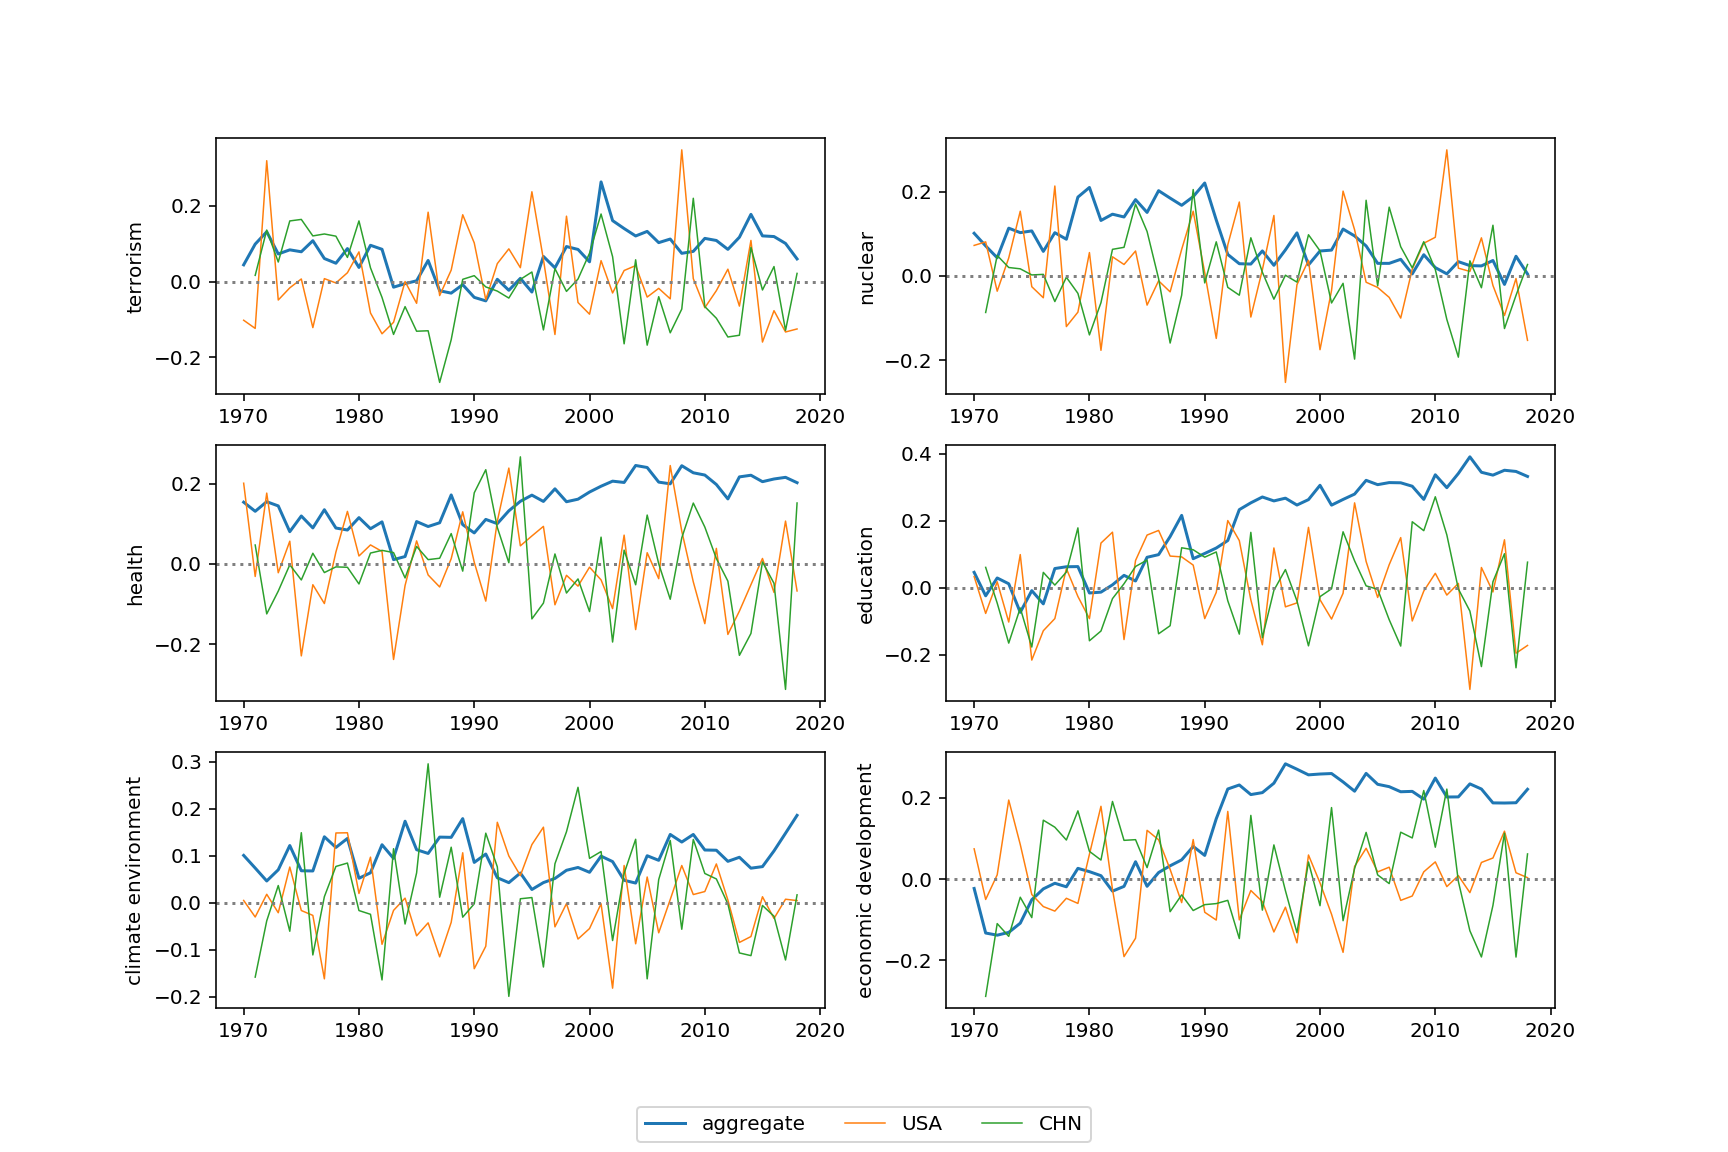
\includegraphics[width=1\textwidth]{graphs/dynamics_attention_on_topics.png}
    \caption{Dynamics of attentions on specific policy issues over years (1970-2018))}
    \label{fig:dynamic attention}
  \end{center}
\end{figure}

As is shown in Figure\ref{fig:dynamic attention}, health, education, climate change, and economic development received substantial attention by the international society in recent decades. This can be largely explained by the efforts promoted by the United Nations on these issues. The graph shows a sharp increase of the international attention on terrorism in the year of 2001, suggesting the escalated concerns and tensive discussions about this topic after the Septembere 11 attack happend in New York. As for the nuclear weapon issue, the international attention calmed down after 1991 when the Soviet Union collapse and the Cold War terminates. 

Among these topics, there is no significant emphasis put by the US or China. Even though the international society has shown constantly increasing concerns about health, education, climate change, and economic development, the attentions paid by the US and China shift back and forth around zero cosine similarity on these topics. However, this may not necessarily suggest that the US and China do not prefer discussions or international efforts on such topics. On the contrary, this may be explained by the diversity of the statements made by the two countries each year. Due to time limitations on the General Debate section, states concerning a wide range of issues must have shortened the length of speech on specific topics. We can verify this by looking back at the original scripts of US statements. Nevertheless, it is still obvious that the dynamics of the US and China's concerns on these topics are highly correlated to that of the international society, which indicates the significant role played by the two countries in the UNGA conference. 

\subsection{Policy Position Proximity and International Relations}

Given the complexity of state policy objectives and the international relations, it is beneficial to investigate state policy positions in high dimensions. We first assume that the policy positions are expressed in the General Debate statemetns and can be represented by the TF-IDF matrix. Then we turn to more sophisticated models to reveal similarities and discrepencies between state policy positions including the Doc2Vec semantic space and the LDA topic modeling. 

\begin{figure}[ht!]
  \begin{center}
    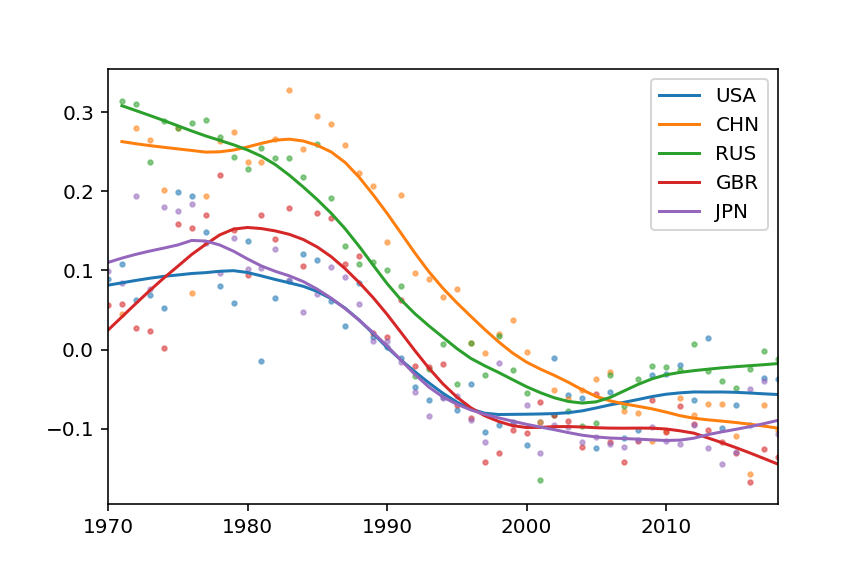
\includegraphics[width=0.8\textwidth]{graphs/tfidf_pca_1.png}
    \caption{Multi-dimensional policy position revelation: principle component of the TF-IDF matrix (1970-2018))}
    \label{fig:tfidf pca 1}
  \end{center}
\end{figure}

To characterize high-dimensional state policy positions, we perform Principle Components Analysis on the TF-IDF matrix, which decomposes the TF-IDF vectors for each document to a scalar that accounts for the most variation in the data. In Figure\ref{fig:tfidf pca 1}, we visualize the results for the US, China, Russia (previously the Soviet Union), the UK, Japan, Korea, and the European Union to make a shallow observation of the international relations revealed by the TF-IDF matrix. It is obvious that, before 1990, China and Russia are similar to each other in terms of policy positions, and the US is closer to the UK and Japan. This is consistent with the historical context. While the Sino-soviet split from 1956 to 1966 is not captured by our data, the improvement of the bilateral diplomatic relationship after that period can be observed from the converging curves of China and the Soviet Union (labelled by RUS) in the figure. The consistency of our results with the history increases our confidence of the validity of our analysis. 

\begin{figure}[ht!]
  \begin{center}
    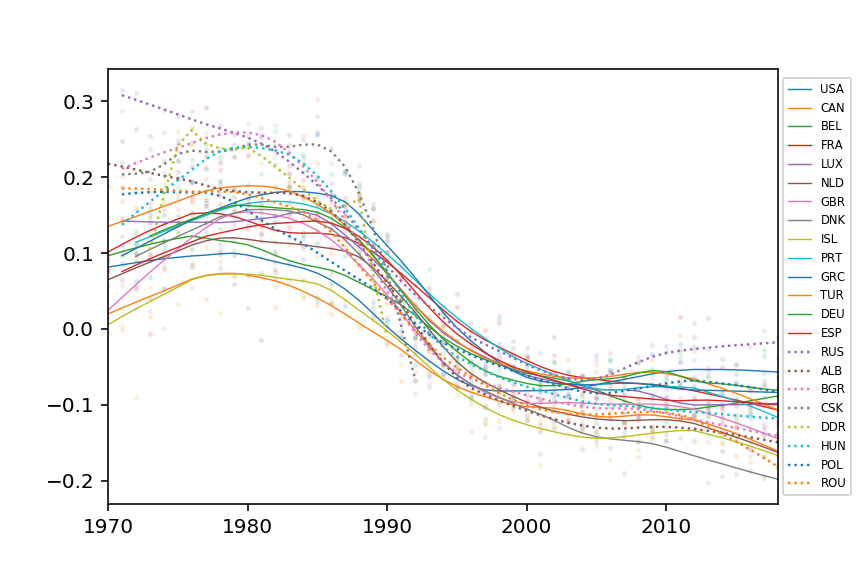
\includegraphics[width=0.8\textwidth]{graphs/tfidf_pca_2.png}
    \caption{Multi-dimensional policy position revelation: NATO and WTO states (1970-2018)}
    \label{fig:tfidf pca 2}
  \end{center}
\end{figure}

We investigate the policy position proximity during the Cold War period. This geopolitical tension mainly between the US and the Soviet Union spaned 45 years before its termination marked by the 1991 dissolution of the Soviet Union \citep{plan80marshall}. We plot the PCA results for all the member states of the North Atlantic Treaty Organization (NATO) and the Warsaw Treaty Organization (WTO in Figure\ref{fig:tfidf pca 2}. The NATO and WTO member states are labelled by the real lines and the dashed lines, respectively. It is a significant pattern that the NATO states and the WTO states show similar policy positions to each other within the organizations before the year of 1990. While the Soviet Union is located on the most extreme position in the figure among other WTO members, the US is laid in the middle of other allies in the NATO. It is also obvious that the discrepencies decrease over years before the dissolution of the Soviet Union. 

Furthermore, we can also conclude that the state policy positions have shown an overall trend of converging in the recent decades, especially by the middle of the 2000s. However, discrepencies seem to have gradually escalated after 2008, the year of the international financial crisis. 

We now turn to the anlysis based on the Doc2Vec semantic space. We examine the cosine similarities between state vectors with the assumption that the policy positions are meaningfully underlying the vector representations of the document in the semantic space. 

\begin{figure}[ht!]
  \begin{center}
    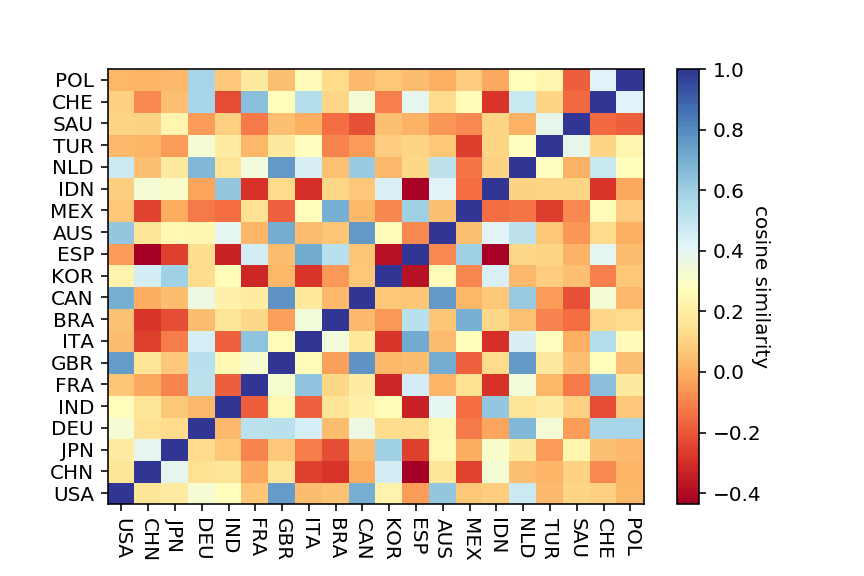
\includegraphics[width=0.8\textwidth]{graphs/doc2vec_consine_similarity_overall.png}
    \caption{Pairwise cosine similarities of 20 states (1970-2018)}
    \label{fig:doc2vec consine overall}
  \end{center}
\end{figure}

In Figure\ref{fig:doc2vec consine overall}, we visualzie the pairwise cosine similarities of the 20 states that have the highest nominal GDP by 2020, according to the IMF. Red cells indicate significant dissimilarities between two states in terms of the meaning of their General Debate statement, and blue cells indicate similarities. Under our assumption, these are equivalent to dispute or disagreement and oncensus or proximiate policy positions, respectively, on policy issues. However, given that the international relations can vary dramatically across time, merely the overall consine similarities cannot capture the dynamics of policy position proximities. 

To examine the dynamics of policy position proximities over years, we calculate the consine similarities between the state vectors each year. As is shown in Figure\ref{fig:doc2vec consine average dynamics}, we take the average of the results within every five years from 1970 to 2015 to cancel out noisy variations. The dynamics of recent years is shown individually in Figure\ref{fig:doc2vec consine recent years}. We also visualize the standard deviations of the cosine similarities in Figure\ref{fig:doc2vec consine average dynamics std}. 

Several observations can be made from the figures. First, the UK and the US are consistently similar to each other in terms of policy positions, which conforms to our findings in the previous analysis. Second, the consine similarity between the US and China increase from 1971-1975 to 1976-1980. This can be explained by a series of historical events that mark the improvement of the US-China relations in the 1970s. Starting from 1971, the tension of the US-China relations had been alleviated by a series of civic exchagne activities including the well-known Pingpong diplomacy. In Feburary of 1972, president Nixon's visit to Beijing marks the resumption of the harmonious relations between the two countries, and the US officially changed its diplomatic recognition of China from Taipei to Beijing on January 1, 1979. Besides, there are also significant results that can hardly be explained by the history. For example, while the figure suggests significant dissimilarities between Spain and French, and French and India, we cannot match any important historical events to the analytical results. 

Again, we apply this analysis to examine the Cold War period. We train the Doc2Vec model again using the 1970-1991 subset of the UNGDC corpus (see Figure\ref{fig:doc2vec semantic space cold war}). In Figure\ref{fig:doc2vec projection cold war}, all the states in our corpus are projected onto a basis vector constructed by the difference of the mean of the NATO state vectors and the WTO state vectors as well as the tokens "capitalism" and "socialism". NATO and WTO member states are indicated by bigger labels. Blue labels indicate proximity to the NATO camp, and red labels indicate proximity to the WTO camp. Only the related positions on the north-to-south direction is meaningful, and horizontal variations are randomly assgined to make a clear visualization. This result is a simple prediction of whether a state is closer to the NATO camp or to the WTO camp before the dissolution of the Soviet Union. 

\begin{figure}[ht!]
  \begin{center}
    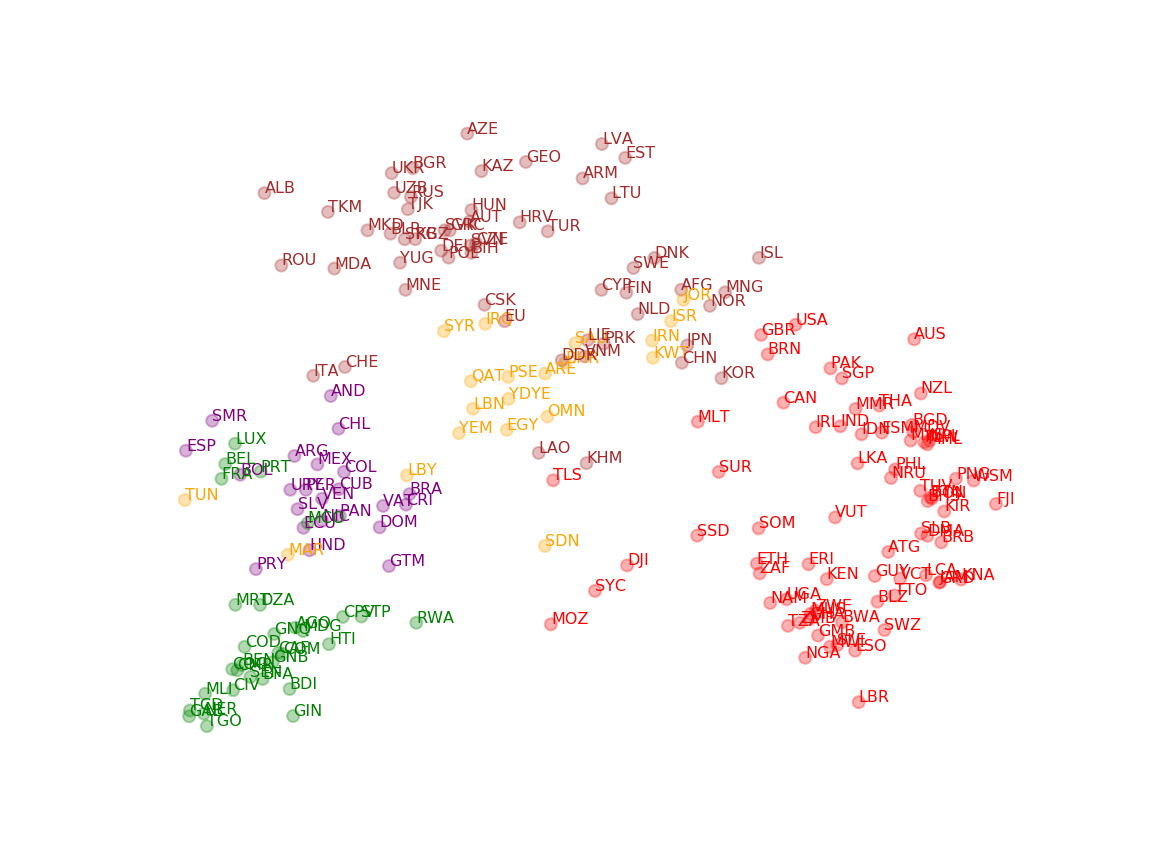
\includegraphics[width=0.8\textwidth]{graphs/doc2vec_kmeans_clustering.png}
    \caption{K-means clustering of Doc2Vec state vectors}
    \label{fig:doc2vec clustering}
  \end{center}
\end{figure}

We finally perform K-means clustering on the Doc2Vec state vectors. The result is shown in \ref{fig:doc2vec clustering}. After tunning the parameter, the optimal number of clusters is 5, which means the states can be optimally partitioned into five state blocs. As is shown in Table\ref{tab:doc2vec clustering}, the top states listed in cluster 0, Austrialia (AUS), Canada (CAN), the UK (GBR), Ghana (GHA), the Gambia (GMB) are members of the Commonwealth of Nations. The top states in cluster 2 are mostly South American countries, and cluster 3 mainly involves middle eastern countries. The result is correlated to the status quo of the geopolitical structure of the world. It identifies latent state blocs in terms of policy position proximities. 

[mutual information network]

\section{Reflections and Extensions}
\label{sec:Reflections and Extensions}

K-means clustering using TF-IDF. No time slice, features are assoicated with single document, which is the distinguishing features of the specific state in the specific year. 

\bibliographystyle{elsarticle-harv}
\bibliography{reference}

\pagebreak
\appendix
\section{Tables and Graphs}
\begin{table}[ht!]
    \centering
    \caption{Changes of participating states over years}
    \label{state changes}
    \resizebox{\textwidth}{!}{
        \begin{tabular}{rll}
        \toprule
        year &                                               plus &                                              minus \\
        \midrule
        1971 &  IRL LUX POL CHL MLI CHN YDYE CAF BFA MUS PAN M... &                                        HND CRI GMB \\
        1972 &    MWI HND SWZ CRI DNK ARE BTN GMB BHR OMN BRB PRT &                                        PAN NOR TTO \\
        1973 &                            PAN DEU BHS LSO DDR NOR &        MWI DOM SWZ GMB CIV UGA TGO MLT CMR TCD BRB \\
        1974 &  DOM SWZ GMB BGD GRD CIV GNQ UGA BWA TGO MLT CM... &                                PAN FJI ZAF BHS MDG \\
        1975 &                                MOZ PAN MWI FJI MDG &                    LBN LUX SWZ GMB HTI CIV EGY MLT \\
        1976 &        LBN CPV SWZ MDV PNG COM GNB STP EGY MLT SUR &                                        MWI GNQ THA \\
        1977 &            MWI LUX AGO WSM GMB TTO HTI CIV SYC THA &                                    GUY DOM GAB MLT \\
        1978 &                            DOM GNQ GAB VNM MLT GUY &                                MWI SWZ PRY GIN SAU \\
        1979 &                        DJI MWI DMA PRY VAT GIN SAU &                                    GMB DNK SWE AGO \\
        1980 &                SWZ LCA VCT AGO DNK SWE GMB BHS ZWE &                                    KWT WSM DMA VAT \\
        1981 &                                        KWT WSM DMA &                        NOR MWI SWZ MMR GMB TTO LSO \\
        1982 &                        NOR ATG MMR GMB TTO BLZ LSO &                                LBN DMA WSM CIV SYC \\
        1983 &                                LBN VUT SLB WSM SYC &                                        PAN LCA GMB \\
        1984 &                            PAN SWZ LCA DMA GMB ZAF &                                VCT WSM GRD SYC ZMB \\
        1985 &                                    MWI WSM BRN KNA &  LBN CPV ATG SEN LCA DMA MDV BTN GMB GNB FJI GN... \\
        1986 &  LBN CPV ATG SEN VCT MDV BTN GMB GNB GRD FJI GN... &                                    MDG UGA BEN KNA \\
        1987 &                                BEN LCA KNA GAB MDG &                                            STP ATG \\
        1988 &                                        STP ATG UGA &                                                GUY \\
        1989 &                                    GUY CIV SYC DMA &                                LBN SLE WSM BTN CAF \\
        1990 &                        LBN SLE WSM BTN LIE CAF NAM &                                   YDYE STP KHM CIV \\
        1991 &            EST KOR PRK LTU LVA FSM CIV STP MHL KHM &                                    COD DDR NER SOM \\
        1992 &  TJK BIH KGZ MDA HRV SVN NER GEO SMR ARM UZB AZ... &                LCA WSM TTO CAF KHM ZMB GUY YUG THA \\
        1993 &  LCA WSM TKM MKD CZE TTO CAF SVK KHM ERI GUY MC... &                                VUT GEO STP CSK MDG \\
        1994 &                                GEO ZAF ZMB MDG AND &                                            WSM TKM \\
        1995 &                                            WSM TKM &                    CPV DMA COM CIV UZB SYC ZWE SAU \\
        1996 &            CPV VUT DMA COM PLW CIV UZB SYC ZWE SAU &                                                CMR \\
        1997 &                                                    &                                WSM PLW FSM KHM SAU \\
        1998 &                            WSM FSM PSE STP CMR SAU &                                                MHL \\
        1999 &                                        PLW KHM MHL &                                        CAF SYC STP \\
        2000 &                                        CAF NRU SOM &                            MOZ WSM BTN CMR UZB ZMB \\
        2001 &        MOZ WSM TON BTN STP ZMB CMR UZB TUV SYC YUG &                                                    \\
        2002 &                                                CHE &                                            LBY SYC \\
        2003 &                                        KIR TLS SYC &                                            DJI TKM \\
        2004 &                                    DJI VAT TKM LBY &                                                SOM \\
        2005 &                                                SOM &                    DJI HND MLI LBR BWA SYC SAU OMN \\
        2006 &                SRB HND MNE MLI LBR BWA SYC SAU OMN &                                                YUG \\
        2007 &                                                    &                                            SAU MLI \\
        2008 &                                                MLI &                                                    \\
        2009 &                                                DJI &                                                    \\
        2010 &                                                    &                                    DJI MDG UZB TKM \\
        2011 &                             DJI SSD TKM UZB EU MDG &                                                SYC \\
        2012 &                                            SAU SYC &                                                GNB \\
        2013 &                                                GNB &                                        DJI KEN SAU \\
        2014 &                                                KEN &                                                    \\
        2015 &                                            DJI SAU &                                        SGP CMR UZB \\
        2016 &                                        SGP CMR UZB &                                            DJI BRN \\
        2017 &                                            DJI BRN &                                                    \\
        2018 &                                                    &                                                    \\
        \bottomrule
        \end{tabular}
    }
\end{table}

\begin{landscape}
  \begin{table}
    \centering
    \caption{Distinguishing features of K-means cluster centroids}
    \label{tab:kmeans tfidf centroids1}
    \resizebox{1\textwidth}{!}{
        \begin{tabular}{lllllllll}
            \toprule
              Cluster 0 &    Cluster 1 &    Cluster 2 &    Cluster 3 &     Cluster 4 &     Cluster 5 &    Cluster 6 & Cluster 7 &  Cluster 8 \\
            \midrule
                   iraq &    terrorism &       soviet &      morocco &       bahamas &        africa &    guatemala &     sudan &    ecuador \\
                 kuwait &       reform &    socialist &      algeria &          drug &         south &       belize &    malawi &       peru \\
                lebanon &  cooperation &      nuclear &   mauritania &         haiti &       african &   guatemalan &   somalia &      latin \\
                  iraqi &      nuclear &     republic &         arab &     caribbean &       namibia &     american &  ethiopia &   peruvian \\
               lebanese &  afghanistan &  disarmament &      maghreb &         small &  independence &      central &     kenya &   american \\
                   arab &       weapon &     relation &      african &       traffic &        regime &  guatemalans &   eritrea &    america \\
                   iran &   millennium &       weapon &       sahara &        island &      struggle &      america &    somali &  democracy \\
             aggression &    terrorist &  imperialist &       africa &       illicit &     apartheid &    caribbean &    africa &       drug \\
                 israel &      poverty &      detente &      kingdom &  commonwealth &    delegation &         drug &   african &     andean \\
                islamic &  sustainable &        union &  palestinian &         south &      republic &    democracy &      igad &      power \\
            \bottomrule
            \end{tabular}
    }
    \end{table}

    \begin{table}
        \centering
        \caption{Distinguishing features of K-means cluster centroids (continued)}
        \label{tab:kmeans tfidf centroids2}
        \resizebox{1\textwidth}{!}{
            \begin{tabular}{lllllllll}
                \toprule
                   Cluster 9 &    Cluster 10 &  Cluster 11 &     Cluster 12 &  Cluster 13 &   Cluster 14 & Cluster 15 &  Cluster 16 &   Cluster 17 \\
                \midrule
                       japan &         south &     african &          korea &        chad &   azerbaijan &      latin &      guinea &  sustainable \\
                     nuclear &    delegation &      africa &            lao &     chadian &      armenia &      chile &  equatorial &      climate \\
                    japanese &        africa &       congo &         korean &     african &     karabakh &  argentina &       papua &      agendum \\
                  assistance &     operation &    republic &       republic &       libya &     armenian &  venezuela &      bissau &         goal \\
                   operation &       nuclear &     burundi &      peninsula &      africa &  azerbaijani &     brazil &     pacific &       tobago \\
                      weapon &         power &      reform &     democratic &      libyan &      nagorny &     mexico &     african &        woman \\
                      reform &   disarmament &  democratic &        nuclear &    republic &      nagorno &   american &    republic &     trinidad \\
                 disarmament &      relation &     liberia &          north &  delegation &        minsk &    america &      africa &         2015 \\
                       korea &       namibia &   continent &    cooperation &      idriss &         osce &    uruguay &       south &      poverty \\
                      intend &  independence &  delegation &  reunification &      darfur &    armenians &      power &  delegation &         mdgs \\
                \bottomrule
            \end{tabular}
        }
        \end{table}

        \begin{table}
            \centering
            \caption{Distinguishing features of K-means cluster centroids (continued)}
            \label{tab:kmeans tfidf centroids3}
            \resizebox{1\textwidth}{!}{
                \begin{tabular}{lllllllll}
                    \toprule
                      Cluster 18 & Cluster 19 & Cluster 20 &   Cluster 21 &   Cluster 22 & Cluster 23 &   Cluster 24 &   Cluster 25 &   Cluster 26 \\
                    \midrule
                        european &     island &    ukraine &    operation &       israel &    ireland &         arab &       panama &       latvia \\
                          kosovo &   marshall &    georgia &       europe &         arab &      irish &        yemen &        canal &       baltic \\
                           union &    barbuda &  ukrainian &      nuclear &  palestinian &   northern &    terrorism &   panamanian &       reform \\
                          bosnia &    antigua &   georgian &     european &      israeli &    nuclear &      emirate &        latin &      latvian \\
                     herzegovina &      small &   abkhazia &  disarmament &    palestine &   european &      bahrain &     american &     european \\
                          europe &    pacific &    russian &       weapon &       jordan &  operation &        egypt &  panamanians &  sustainable \\
                     cooperation &  caribbean &     russia &  negotiation &    territory &   unionist &  palestinian &      america &  afghanistan \\
                         moldova &    climate &   european &        south &   aggression &    british &       syrian &       treaty &        union \\
                         croatia &    nuclear &     europe &       soviet &       occupy &     weapon &    stability &     republic &       europe \\
                         albania &       test &  chernobyl &          arm &      zionist &   violence &      israeli &      oceanic &        syria \\
                    \bottomrule
                \end{tabular}
            }
        \end{table}

        \begin{table}
            \centering
            \caption{Distinguishing features of K-means cluster centroids (continued)}
            \label{tab:kmeans tfidf centroids4}
            \resizebox{1\textwidth}{!}{
                \begin{tabular}{lllllllll}
                    \toprule
                     Cluster 27 &   Cluster 28 &     Cluster 29 &   Cluster 30 &  Cluster 31 & Cluster 32 &     Cluster 33 &    Cluster 34 & Cluster 35 \\
                    \midrule
                         turkey &      pacific &          spain &     pakistan &    paraguay &  caribbean &        tunisia &       myanmar &   honduras \\
                         cyprus &       island &        spanish &        india &     bolivia &      saint &           arab &          drug &  nicaragua \\
                        turkish &         fiji &      gibraltar &          sri &    bolivian &   barbados &       tunisian &       rakhine &      costa \\
                         greece &      zealand &      operation &        lanka &       latin &    grenada &        maghreb &      narcotic &      haiti \\
                          greek &      solomon &       european &      kashmir &     america &      small &        african &         opium &   salvador \\
                       cypriots &        small &  mediterranean &      nuclear &    american &     island &     solidarity &         poppy &       rica \\
                        cypriot &      climate &         europe &  afghanistan &        drug &   dominica &    palestinian &       nuclear &  dominican \\
                       european &        samoa &       possible &    terrorism &   democracy &      lucia &  mediterranean &        reform &    central \\
                     settlement &       tuvalu &         crisis &       indian &        coca &      kitts &            ben &  constitution &         el \\
                          union &  sustainable &      terrorism &        south &  paraguayan &      haiti &      stability &    democratic &   american \\
                    \bottomrule
                \end{tabular}
            }
        \end{table}
\end{landscape}


\begin{figure}[ht!]
  \begin{center}
    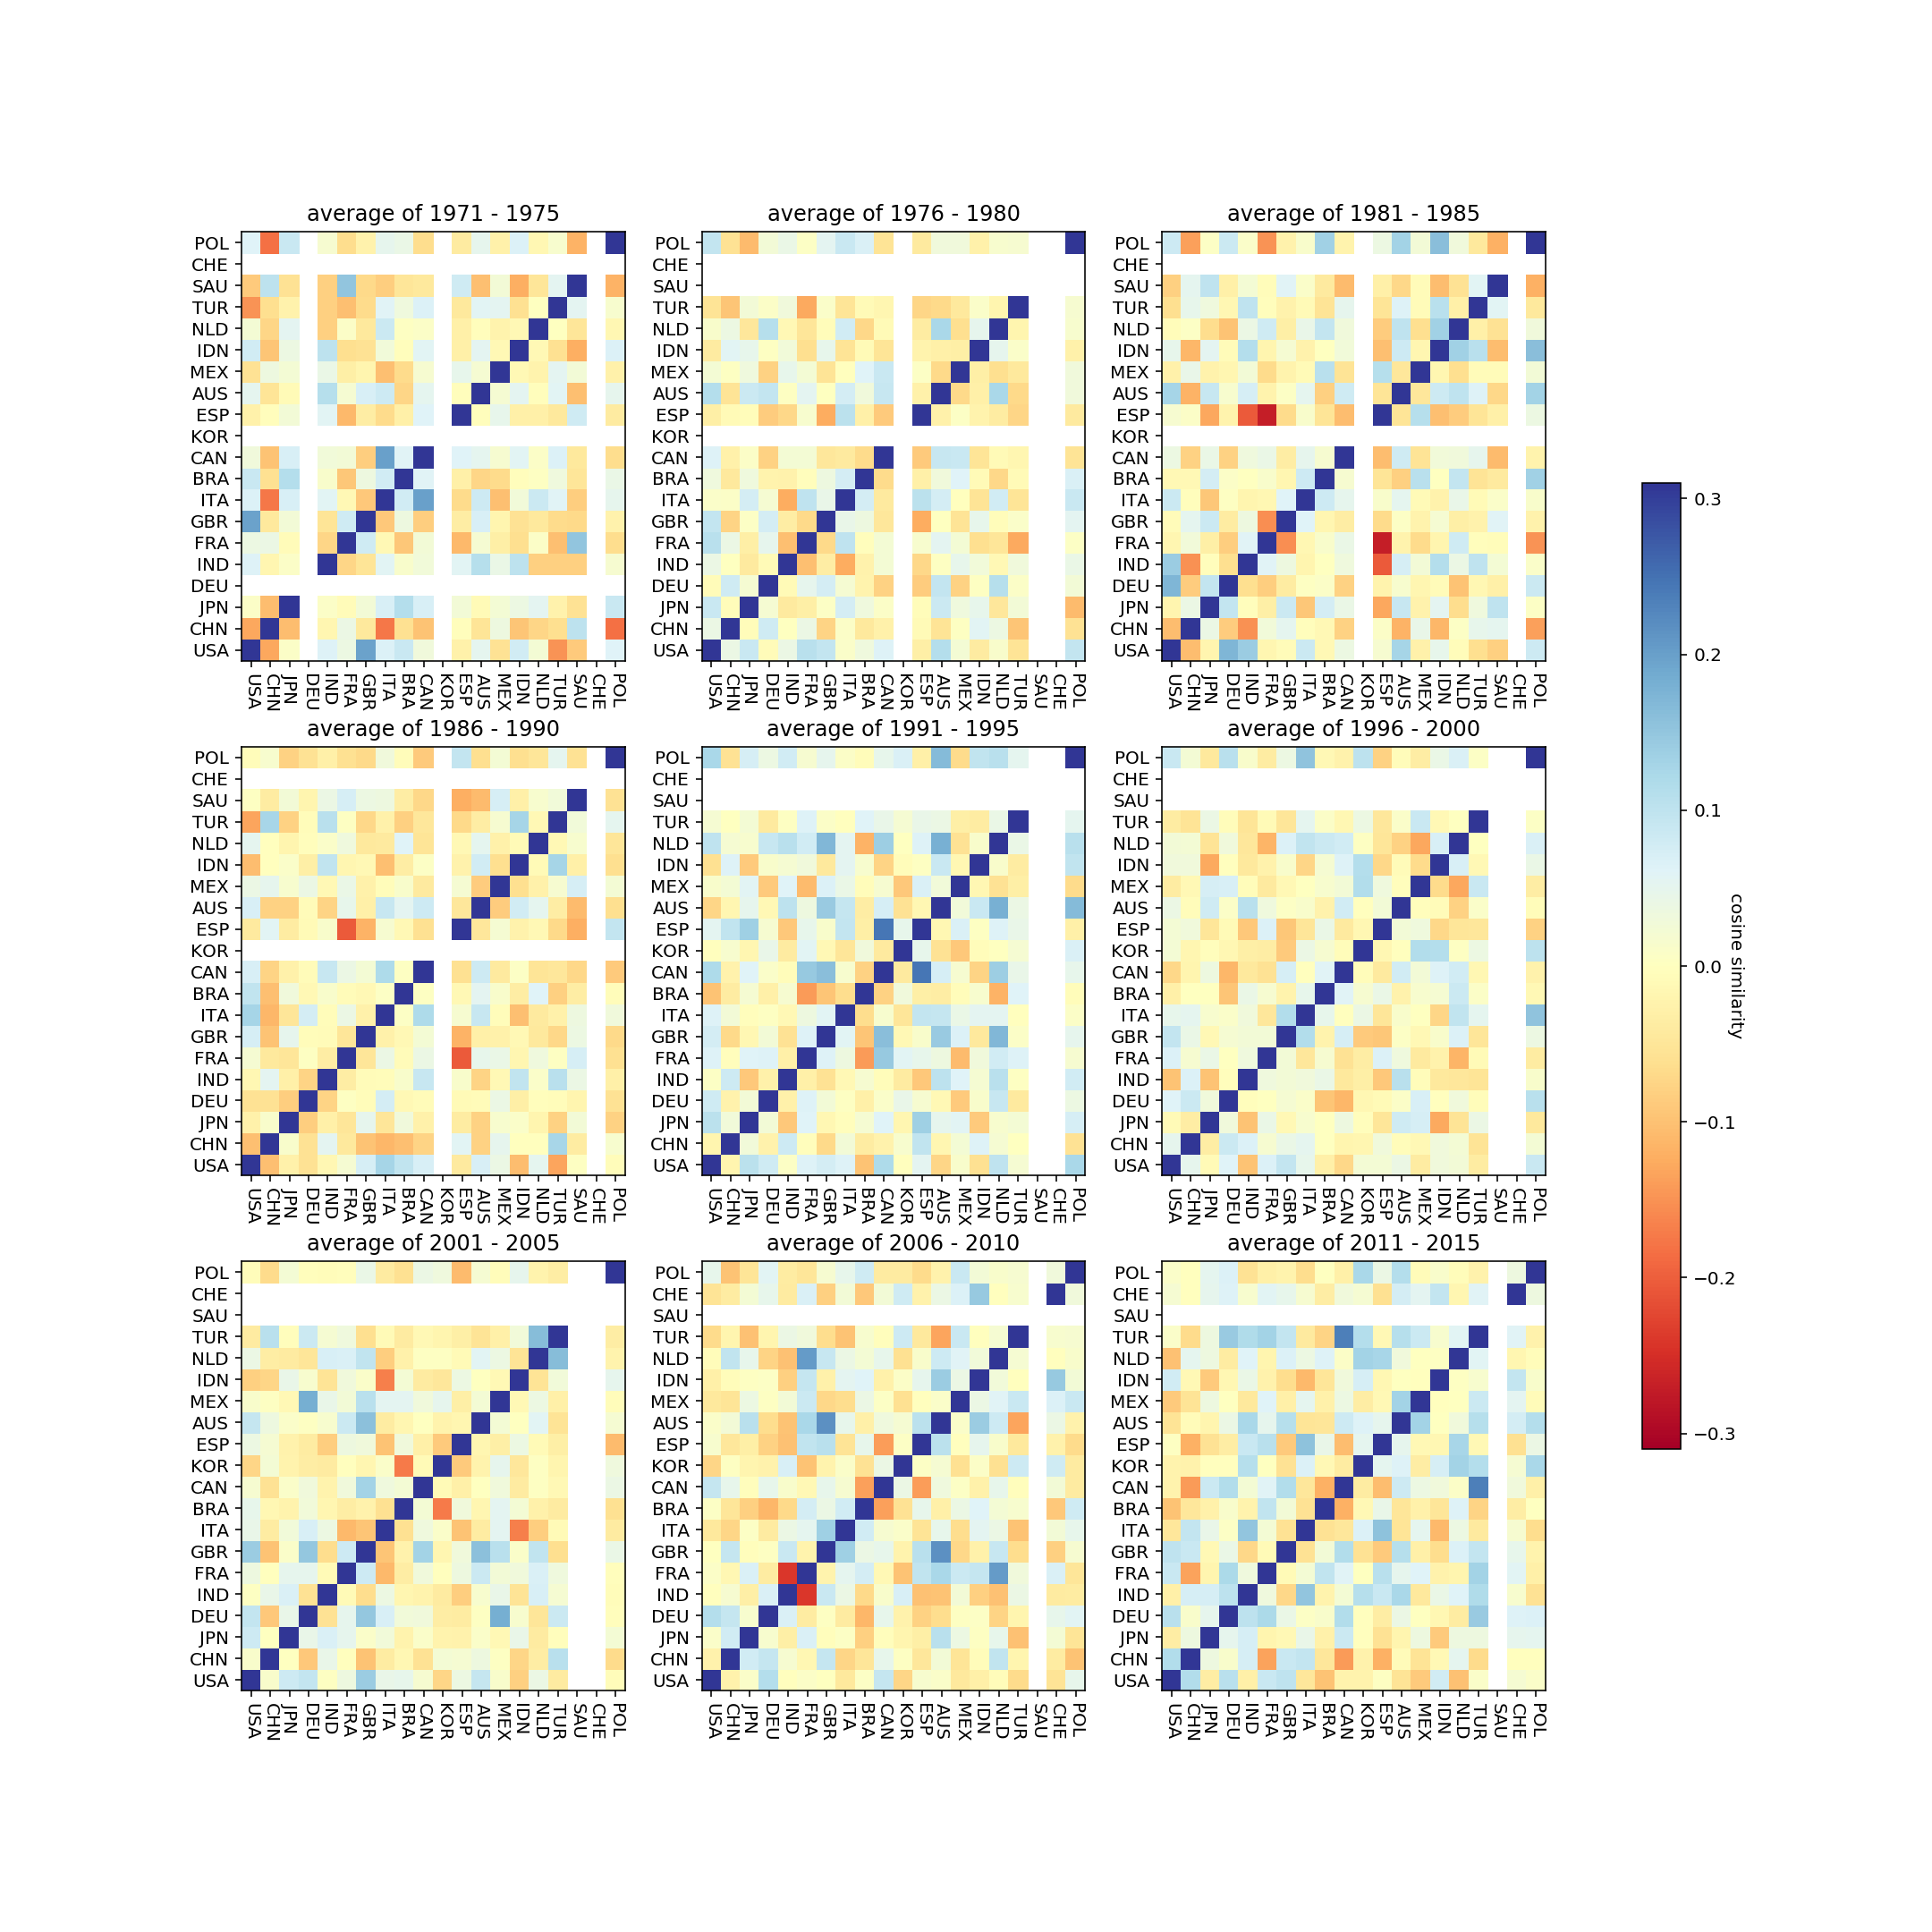
\includegraphics[trim=75 75 75 75, width=\textwidth]{graphs/doc2vec_consine_similarity_average_dynamics.png}
    \caption{Average pairwise cosine similarities of 20 states every five years (1970-2015)}
    \label{fig:doc2vec consine average dynamics}
  \end{center}
\end{figure}

\begin{figure}[ht!]
  \begin{center}
    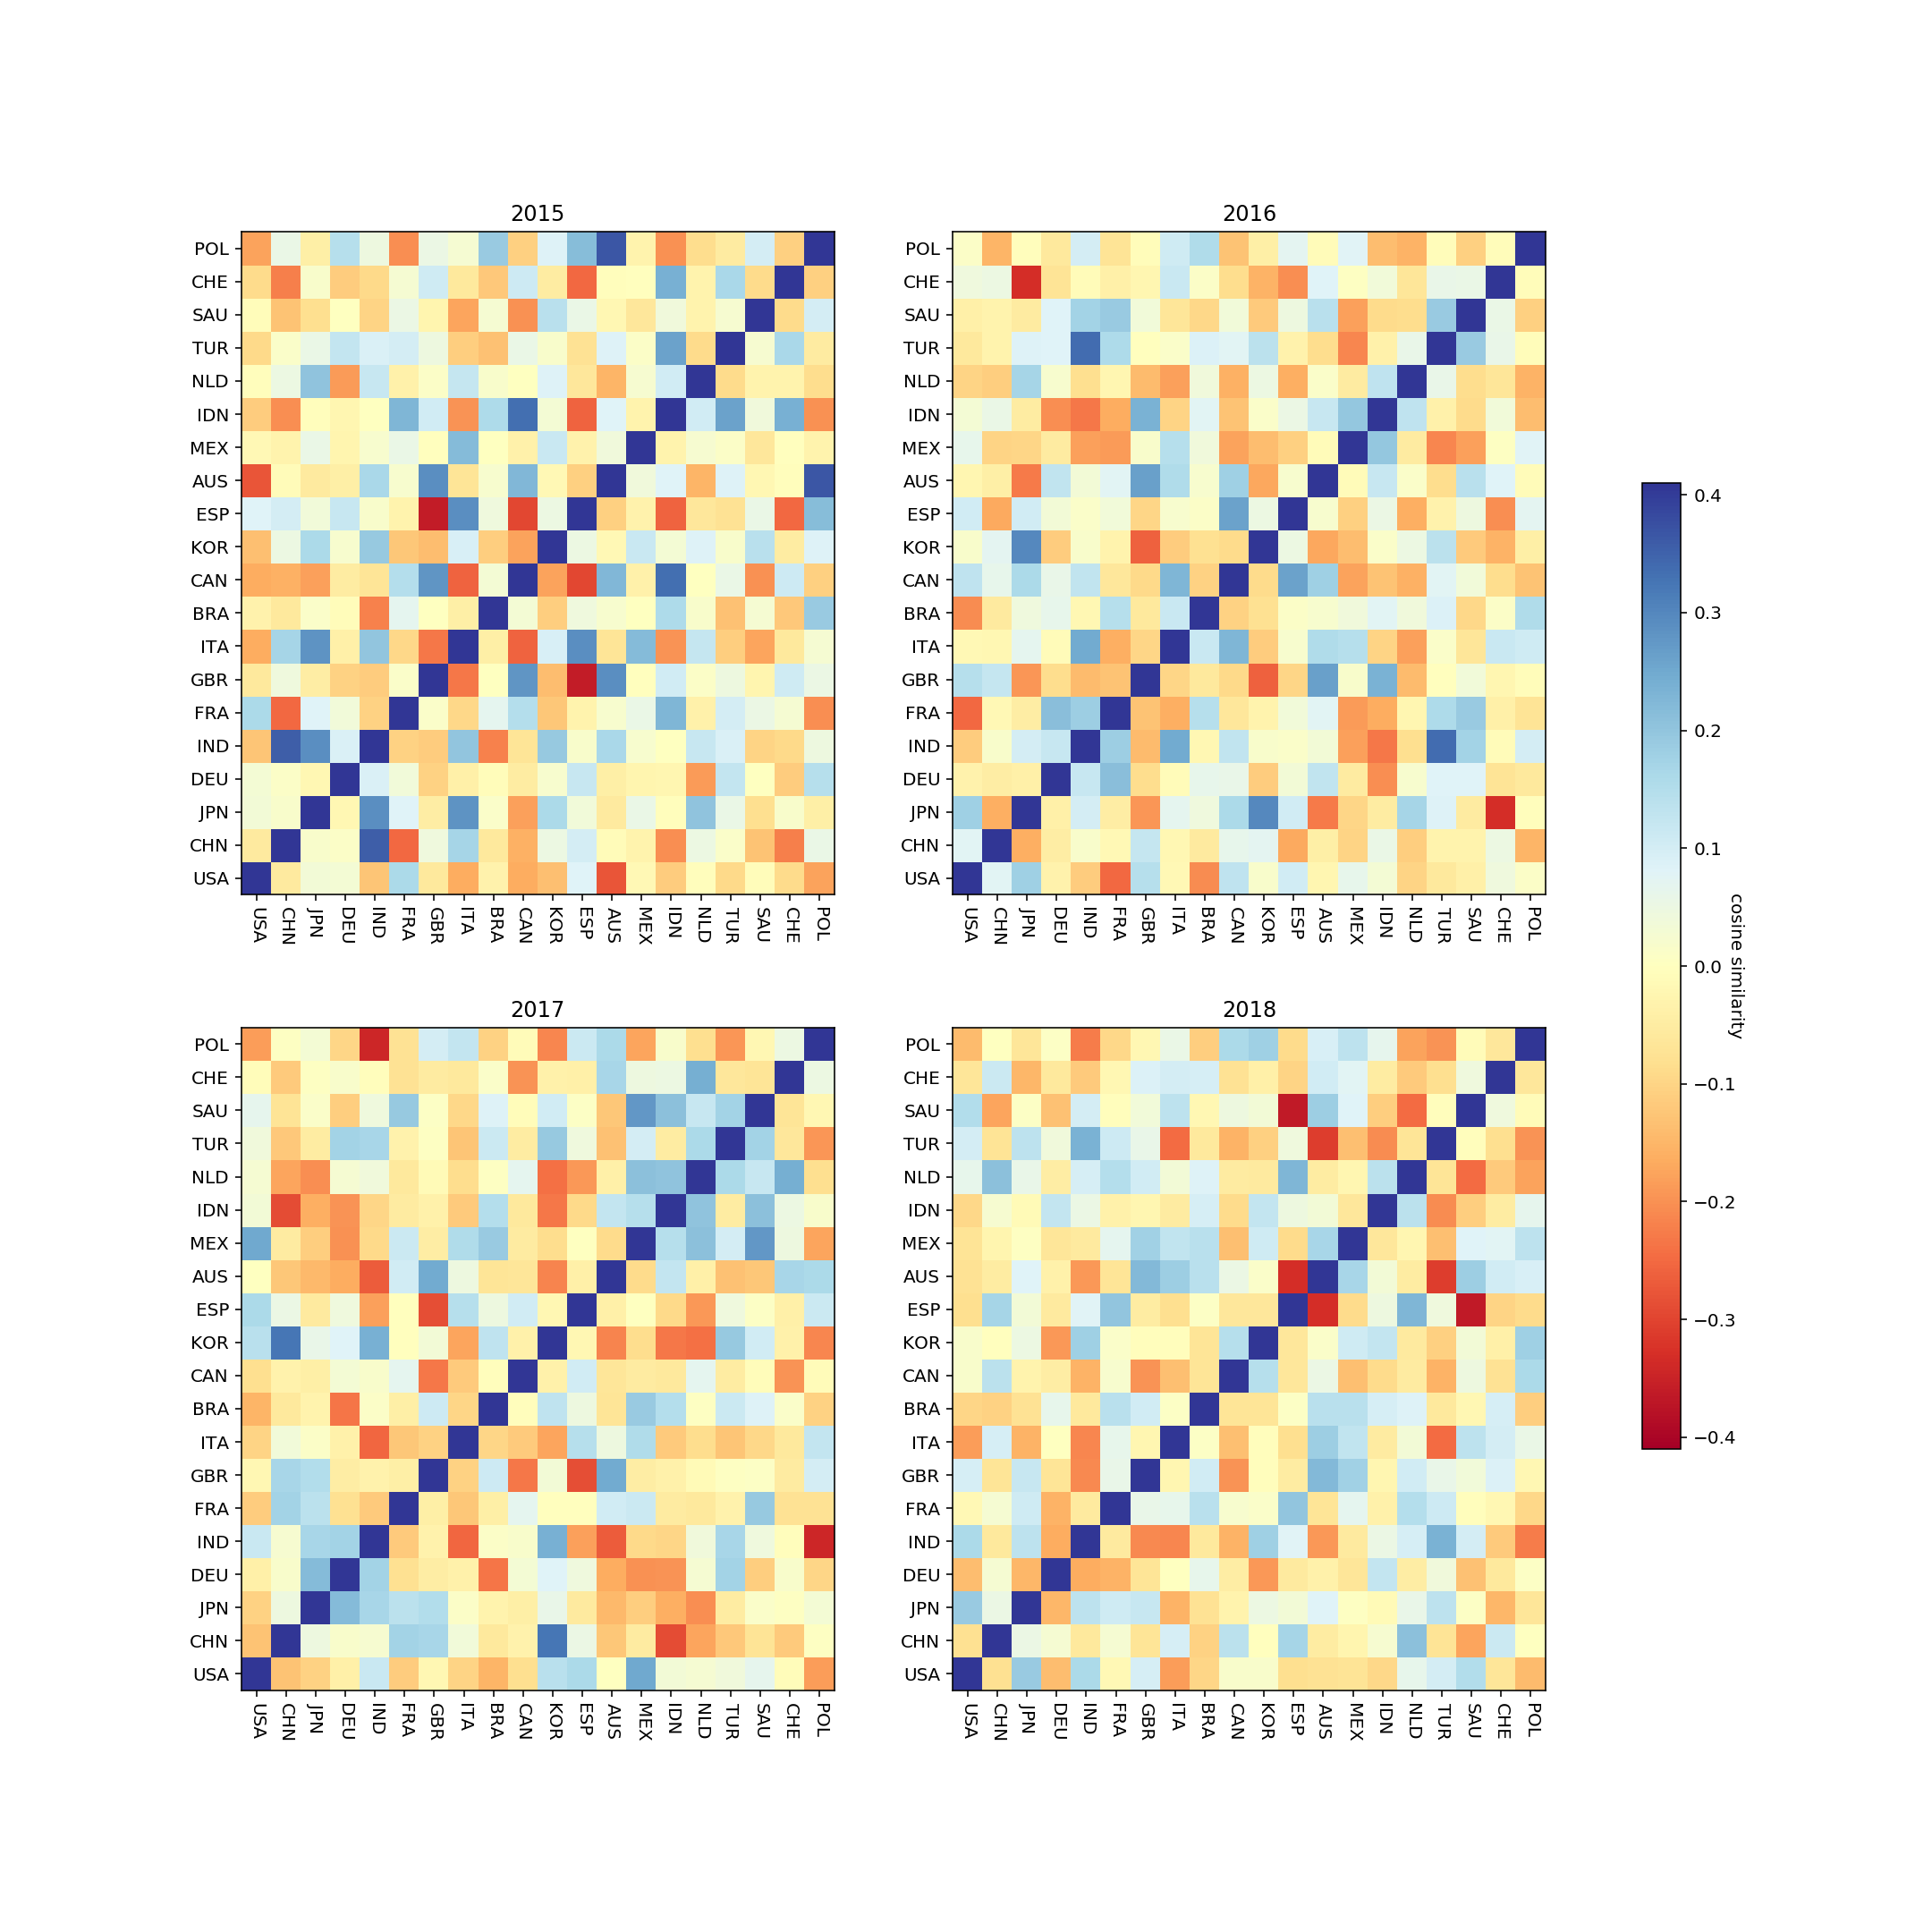
\includegraphics[trim=75 75 75 75, width=\textwidth]{graphs/doc2vec_consine_similarity_recent_years.png}
    \caption{Pairwise cosine similarities of 20 states in recent years (2015-2018)}
    \label{fig:doc2vec consine recent years}
  \end{center}
\end{figure}

\begin{figure}[ht!]
  \begin{center}
    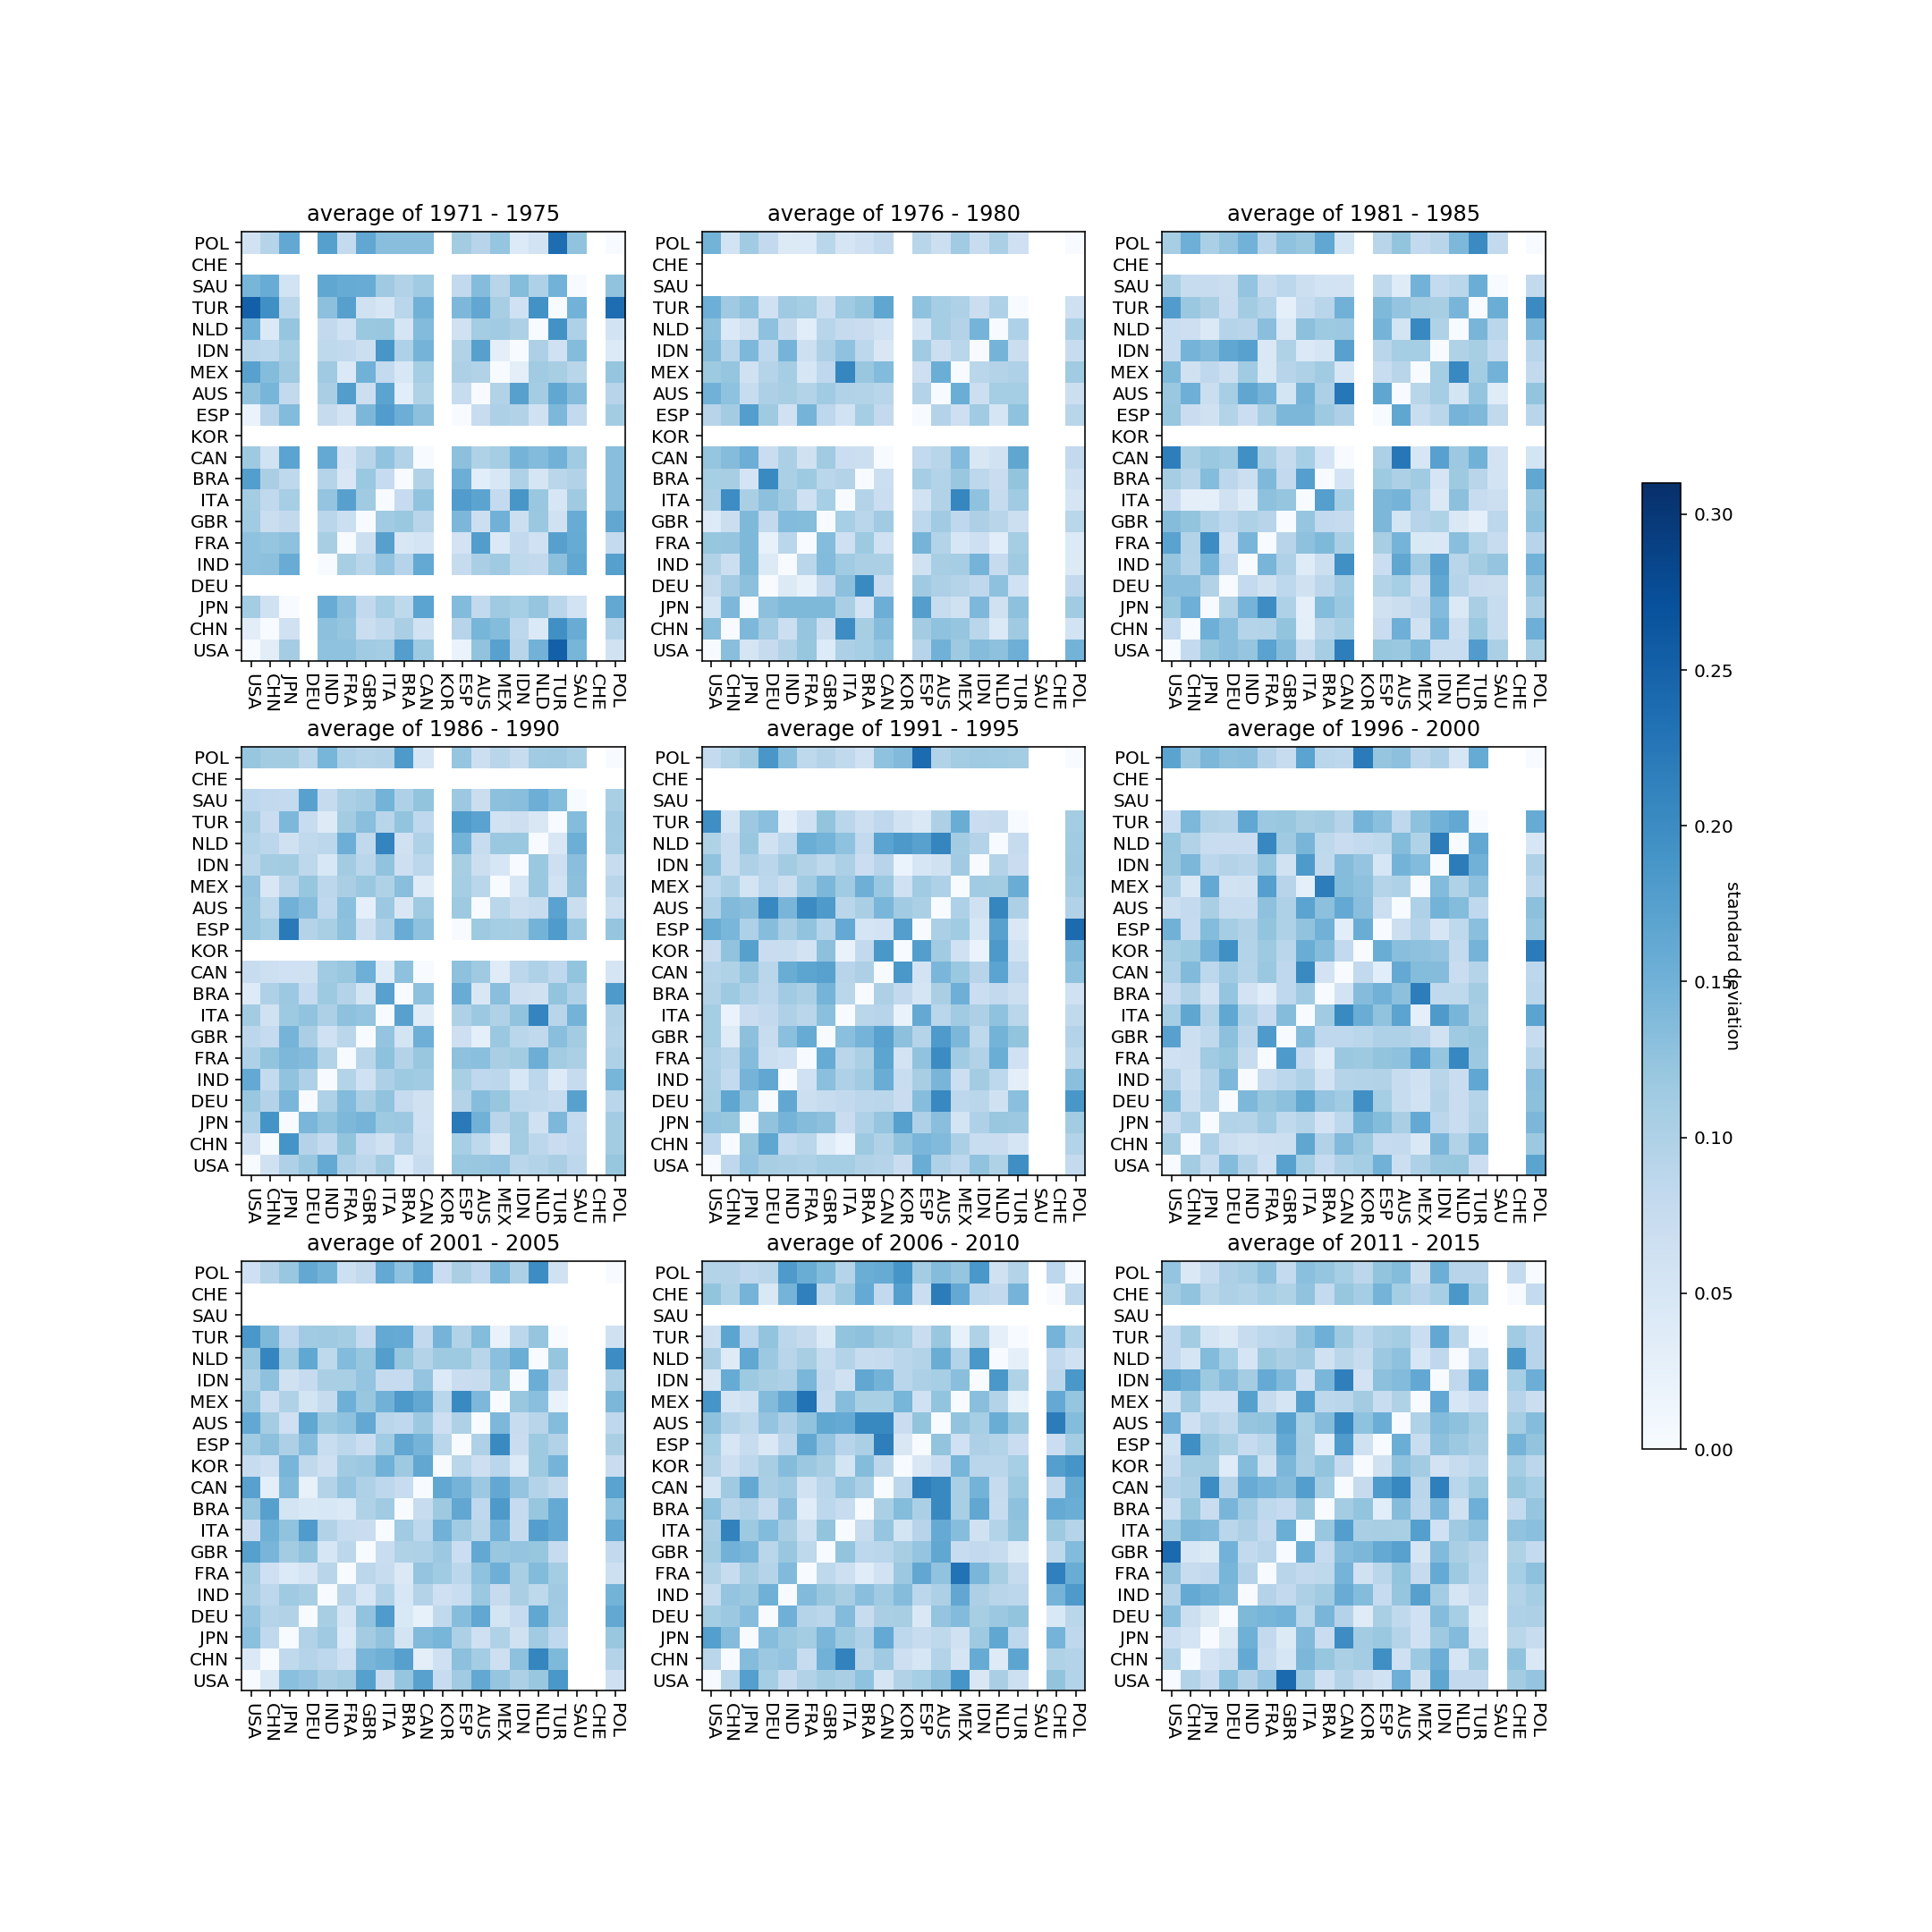
\includegraphics[trim=75 75 75 75, width=\textwidth]{graphs/doc2vec_consine_similarity_average_dynamics_std.png}
    \caption{Standard deviation of pairwise cosine similarities of 20 states every five years (1970-2015)}
    \label{fig:doc2vec consine average dynamics std}
  \end{center}
\end{figure}

\begin{figure}[ht!]
  \begin{center}
    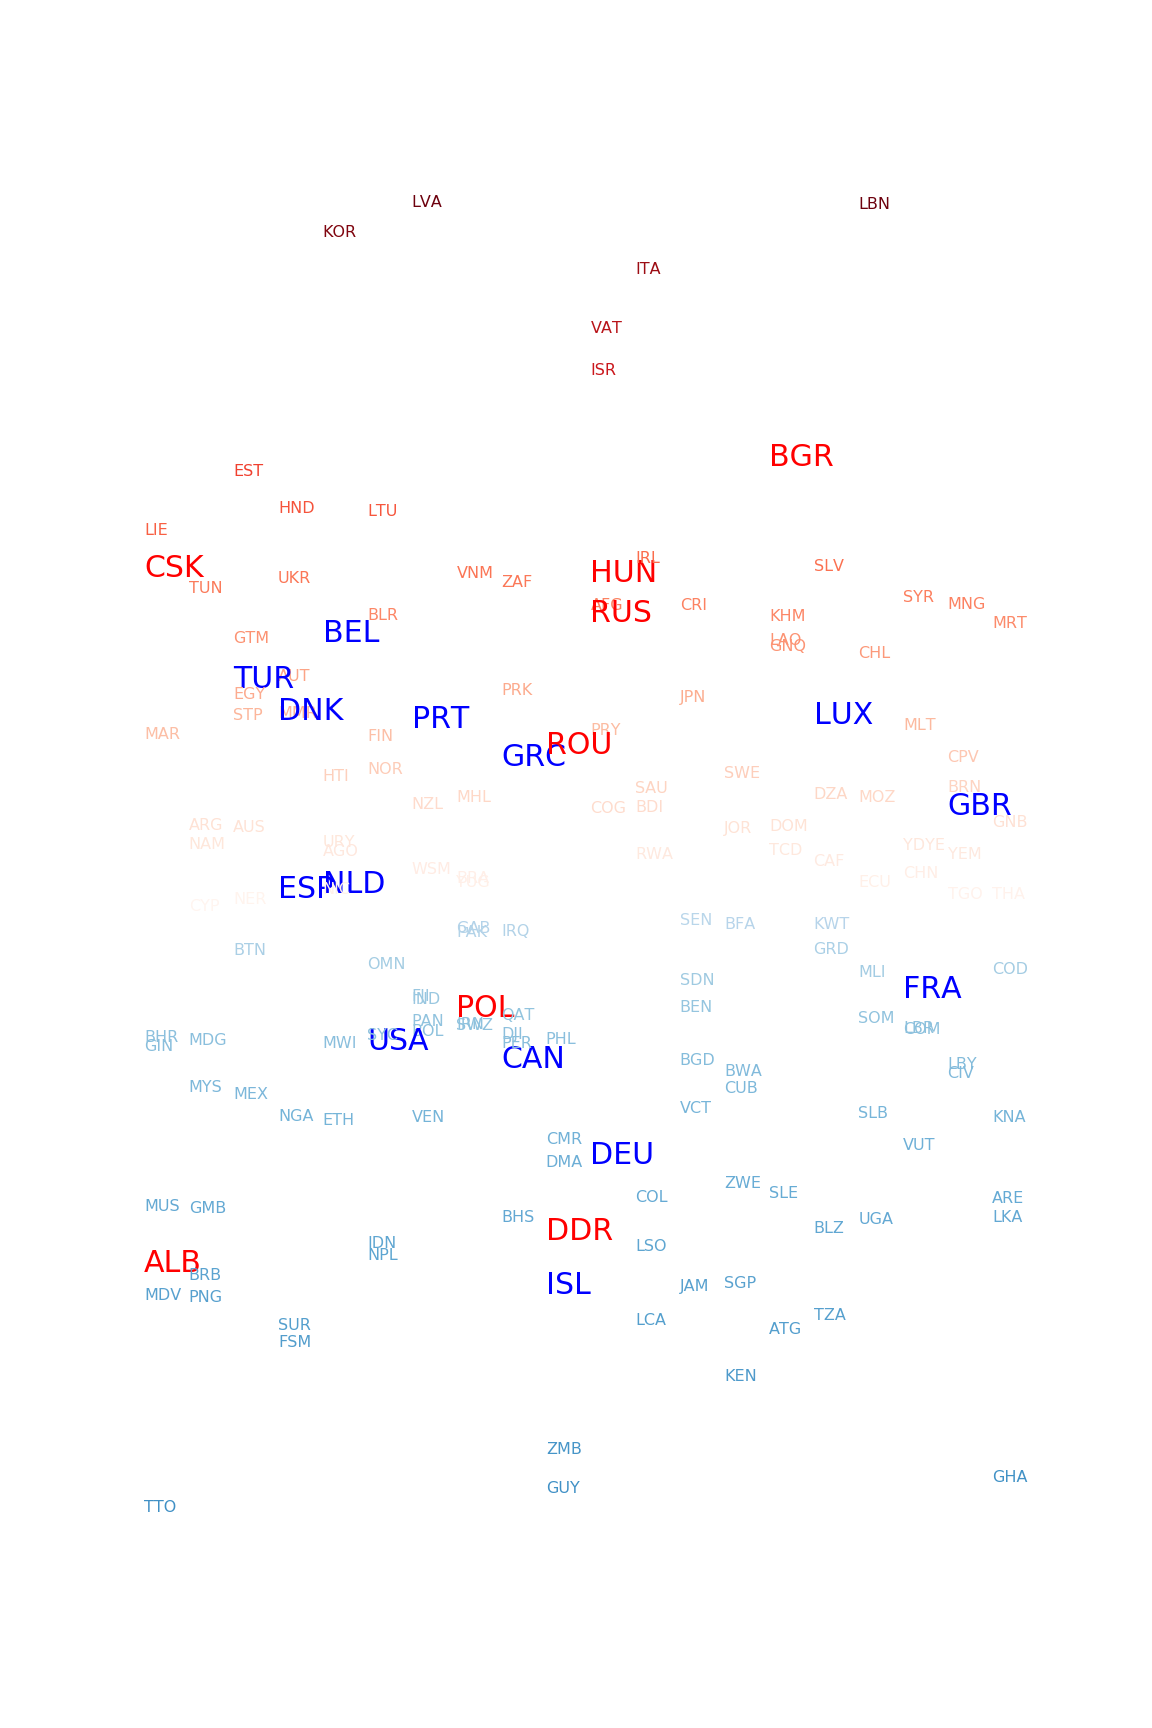
\includegraphics[width=0.8\textwidth]{graphs/doc2vec_projection_coldwar.png}
    \caption{Projection of states vectors onto the Cold War dimension (1970-1991)}
    \label{fig:doc2vec projection cold war}
  \end{center}
\end{figure}

\begin{figure}[ht!]
  \begin{center}
    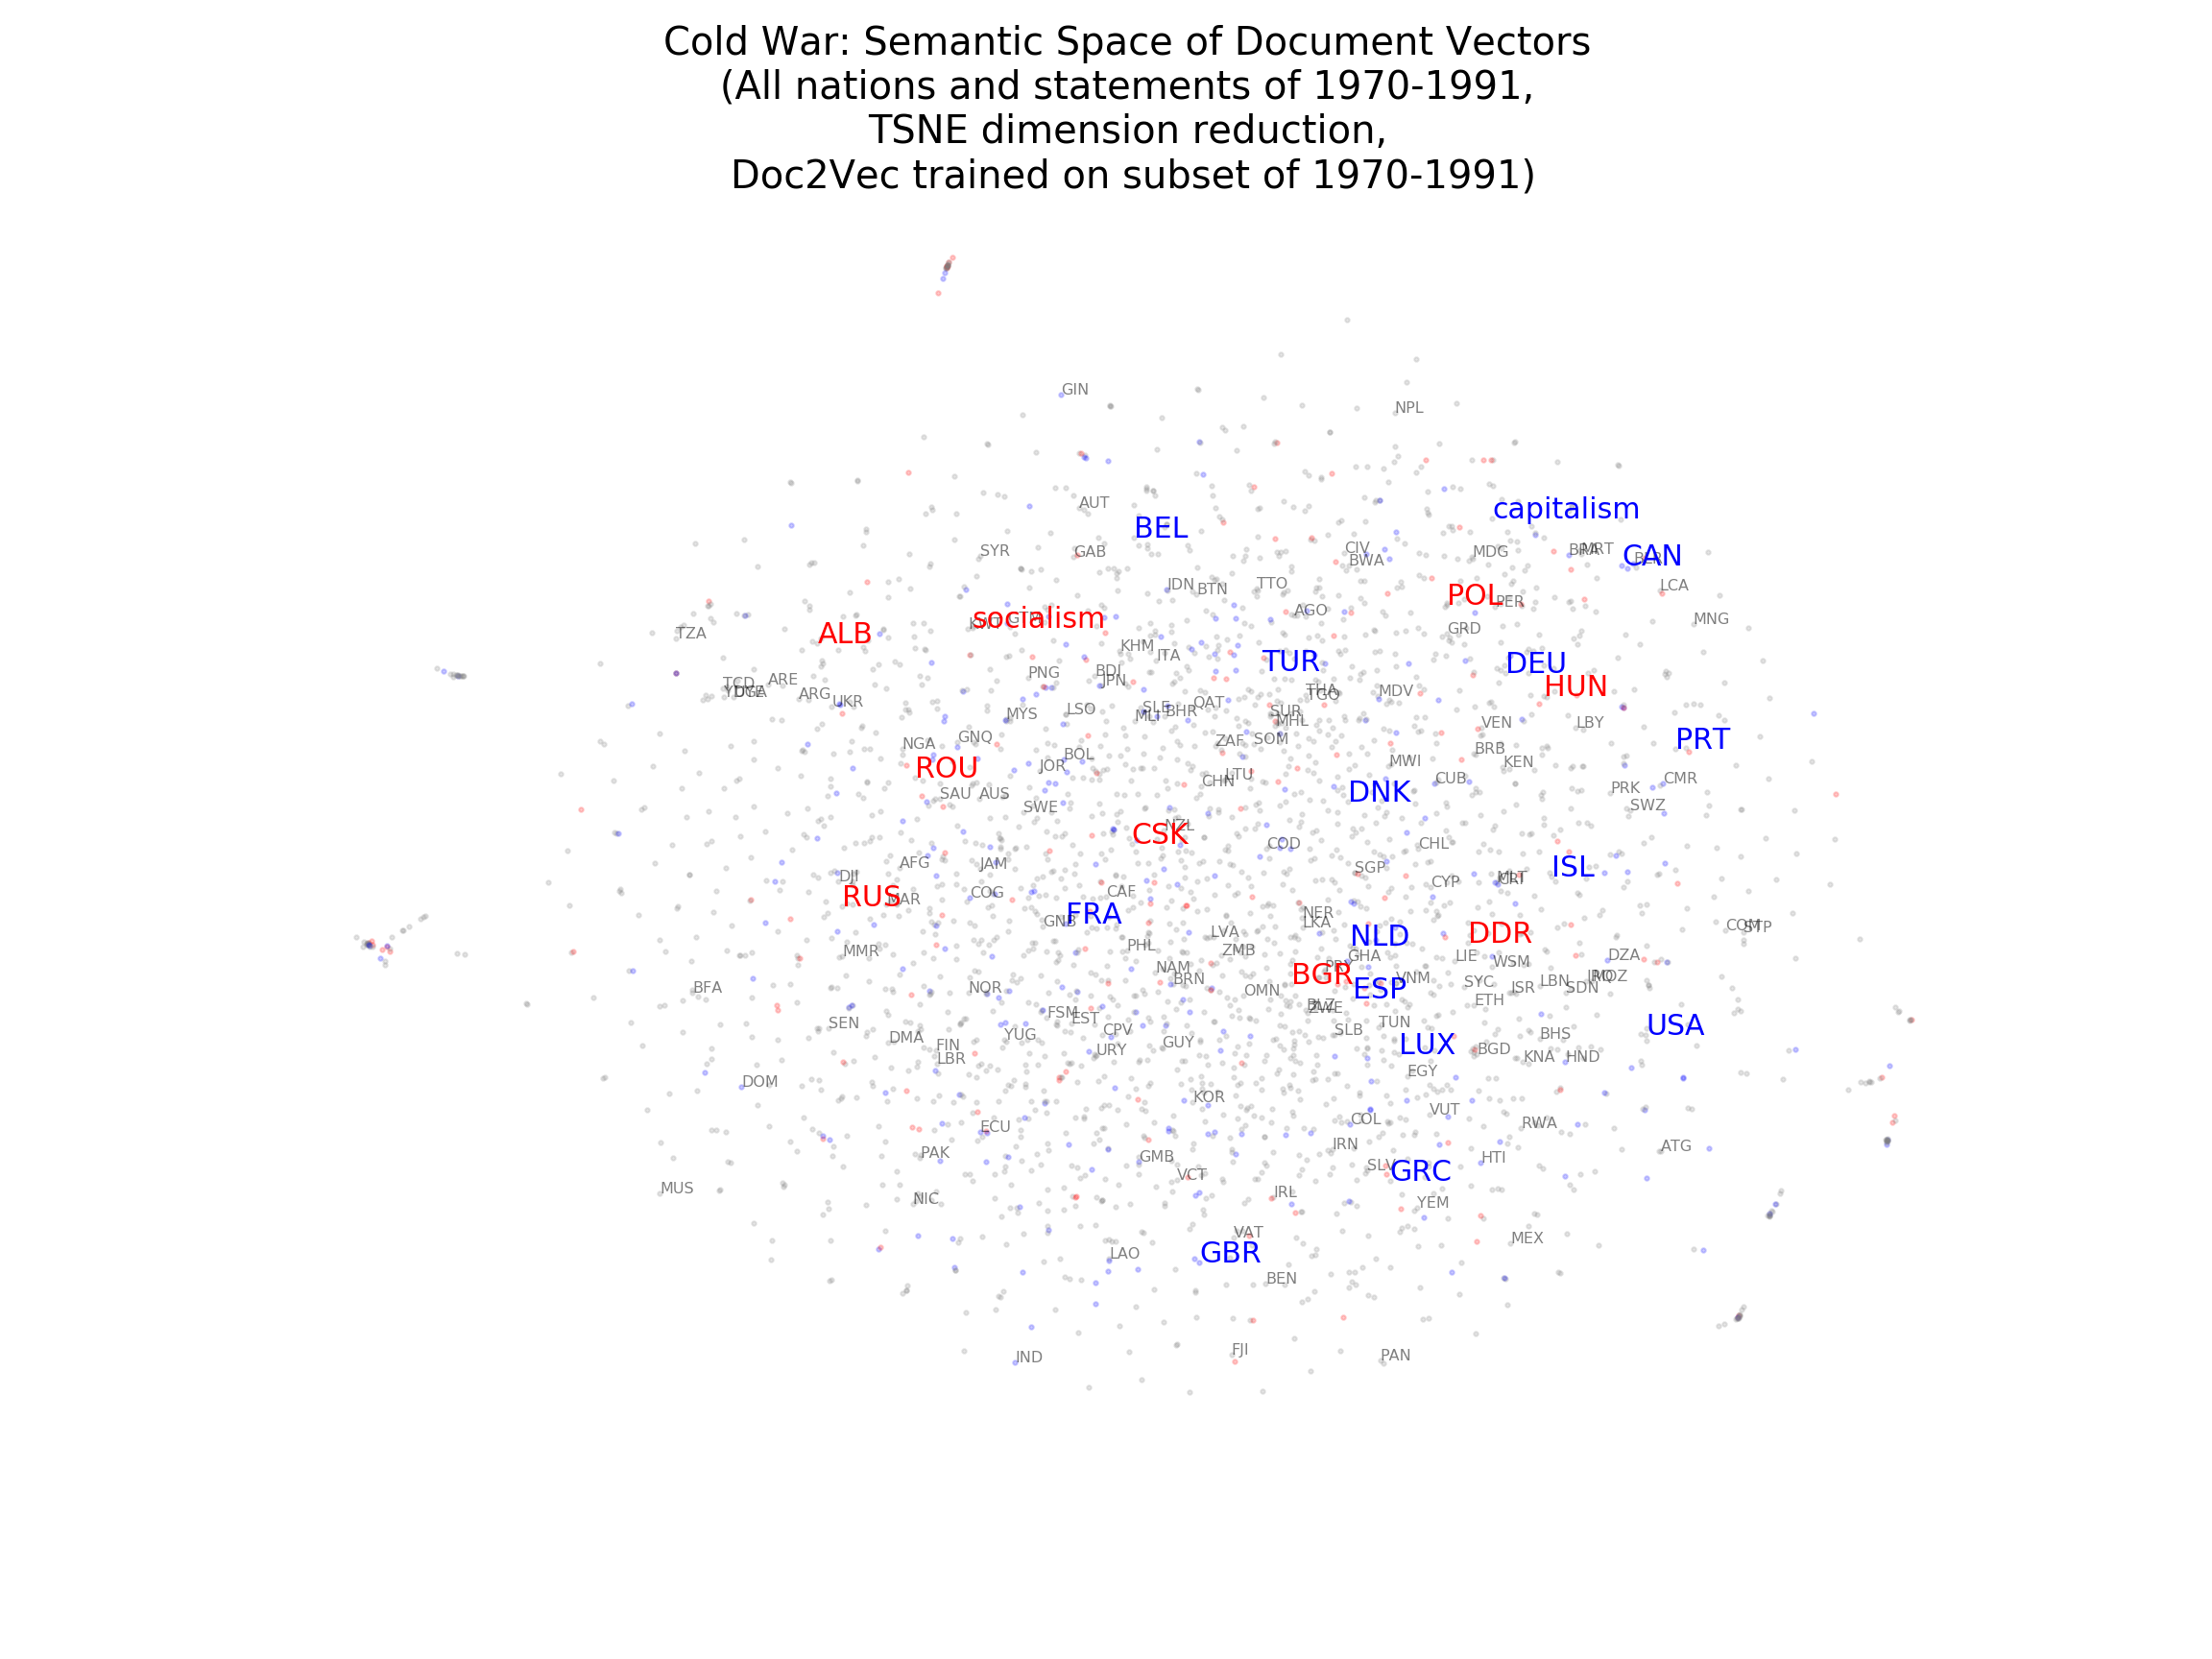
\includegraphics[width=\textwidth]{graphs/doc2vec_semantic_space_cold_war.png}
    \caption{Semantic space of document vectors (1970-1991)}
    \label{fig:doc2vec semantic space cold war}
  \end{center}
\end{figure}

\begin{table}[ht!]
\centering
\caption{K-means clustering of Doc2Vec state vectors}
\label{tab:doc2vec clustering}
\begin{tabular}{lllll}
\toprule
cluster 0 & cluster 1 & cluster 2 & cluster 3 & cluster 4 \\
\midrule
      AUS &       ALB &       ARG &       IRN &       BEL \\
      CAN &       AUT &       BOL &       IRQ &       CMR \\
      GBR &       BLR &       BRA &       ISR &       COG \\
      GHA &       ISL &       COL &       KWT &       DZA \\
      GMB &       ITA &       CRI &       LBN &       FRA \\
      IDN &       JPN &       CUB &       LBY &       GIN \\
      IND &       KHM &       DOM &       MAR &       HTI \\
      KEN &       NLD &       ECU &       SDN &       MDG \\
      LBR &       NOR &       GTM &       SYR &       RWA \\
      LKA &       TUR &       HND &       TUN &       TGO \\
      MMR &       UKR &       MEX &       EGY &       BDI \\
      NZL &       YUG &       PER &       JOR &       BEN \\
      PAK &       AFG &       PRY &       QAT &       BFA \\
      PHL &       BGR &       SLV &       SAU &       CAF \\
      SGP &       CHN &       URY &      YDYE &       CIV \\
      SLE &       CSK &       VEN &       YEM &       COD \\
      SOM &       CYP &       CHL &       ARE &       GAB \\
      THA &       FIN &       ESP &       BHR &       LUX \\
      TTO &       GRC &       NIC &       OMN &       MLI \\
      USA &       HUN &       PAN &       PSE &       MRT \\
      ZAF &       LAO &       VAT &           &       NER \\
      ZMB &       MNG &       SMR &           &       SEN \\
      ETH &       POL &       AND &           &       TCD \\
      FJI &       ROU &           &           &       PRT \\
      GUY &       RUS &           &           &       GNQ \\
      IRL &       SWE &           &           &       COM \\
      JAM &       DNK &           &           &       CPV \\
      MLT &       DDR &           &           &       GNB \\
      MUS &       DEU &           &           &       STP \\
      MYS &       VNM &           &           &       AGO \\
      NGA &       LIE &           &           &       MCO \\
      NPL &       EST &           &           &           \\
      TZA &       KOR &           &           &           \\
      UGA &       LTU &           &           &           \\
      BRB &       LVA &           &           &           \\
      BTN &       PRK &           &           &           \\
      MWI &       ARM &           &           &           \\
      ... &        ...& &&\\
    %   SWZ &       AZE &           &           &           \\
    %   BHS &       BIH &           &           &           \\
    %   LSO &       GEO &           &           &           \\
    %   BGD &       HRV &           &           &           \\
    %   BWA &       KAZ &           &           &           \\
    %   GRD &       KGZ &           &           &           \\
    %   MOZ &       MDA &           &           &           \\
    %   MDV &       SVN &           &           &           \\
    %   PNG &       TJK &           &           &           \\
    %   SUR &       UZB &           &           &           \\
    %   SYC &       CZE &           &           &           \\
    %   WSM &       MKD &           &           &           \\
    %   DJI &       SVK &           &           &           \\
    %   DMA &       TKM &           &           &           \\
    %   LCA &       CHE &           &           &           \\
    %   VCT &       MNE &           &           &           \\
    %   ZWE &       SRB &           &           &           \\
    %   ATG &        EU &           &           &           \\
    %   BLZ &           &           &           &           \\
    %   SLB &           &           &           &           \\
    %   VUT &           &           &           &           \\
    %   BRN &           &           &           &           \\
    %   KNA &           &           &           &           \\
    %   NAM &           &           &           &           \\
    %   FSM &           &           &           &           \\
    %   MHL &           &           &           &           \\
    %   ERI &           &           &           &           \\
    %   PLW &           &           &           &           \\
    %   NRU &           &           &           &           \\
    %   TON &           &           &           &           \\
    %   TUV &           &           &           &           \\
    %   KIR &           &           &           &           \\
    %   TLS &           &           &           &           \\
    %   SSD &           &           &           &           \\
\bottomrule
\end{tabular}

\end{table}


%% The Appendices part is started with the command \appendix;
%% appendix sections are then done as normal sections
%% \appendix

%% \section{}
%% \label{}

%% References
%%
%% Following citation commands can be used in the body text:
%%
%%  \citet{key}  ==>>  Jones et al. (1990)
%%  \citep{key}  ==>>  (Jones et al., 1990)
%%
%% Multiple citations as normal:
%% \citep{key1,key2}         ==>> (Jones et al., 1990; Smith, 1989)
%%                            or  (Jones et al., 1990, 1991)
%%                            or  (Jones et al., 1990a,b)
%% \cite{key} is the equivalent of \citet{key} in author-year mode
%%
%% Full author lists may be forced with \citet* or \citep*, e.g.
%%   \citep*{key}            ==>> (Jones, Baker, and Williams, 1990)
%%
%% Optional notes as:
%%   \citep[chap. 2]{key}    ==>> (Jones et al., 1990, chap. 2)
%%   \citep[e.g.,][]{key}    ==>> (e.g., Jones et al., 1990)
%%   \citep[see][pg. 34]{key}==>> (see Jones et al., 1990, pg. 34)
%%  (Note: in standard LaTeX, only one note is allowed, after the ref.
%%   Here, one note is like the standard, two make pre- and post-notes.)
%%
%%   \citealt{key}          ==>> Jones et al. 1990
%%   \citealt*{key}         ==>> Jones, Baker, and Williams 1990
%%   \citealp{key}          ==>> Jones et al., 1990
%%   \citealp*{key}         ==>> Jones, Baker, and Williams, 1990
%%
%% Additional citation possibilities
%%   \citeauthor{key}       ==>> Jones et al.
%%   \citeauthor*{key}      ==>> Jones, Baker, and Williams
%%   \citeyear{key}         ==>> 1990
%%   \citeyearpar{key}      ==>> (1990)
%%   \citetext{priv. comm.} ==>> (priv. comm.)
%%   \citenum{key}          ==>> 11 [non-superscripted]
%% Note: full author lists depends on whether the bib style supports them;
%%       if not, the abbreviated list is printed even when full requested.
%%
%% For names like della Robbia at the start of a sentence, use
%%   \Citet{dRob98}         ==>> Della Robbia (1998)
%%   \Citep{dRob98}         ==>> (Della Robbia, 1998)
%%   \Citeauthor{dRob98}    ==>> Della Robbia


%% References with bibTeX database:


%% Authors are advised to submit their bibtex database files. They are
%% requested to list a bibtex style file in the manuscript if they do
%% not want to use elsarticle-harv.bst.

%% References without bibTeX database:

% \begin{thebibliography}{00}

%% \bibitem must have one of the following forms:
%%   \bibitem[Jones et al.(1990)]{key}...
%%   \bibitem[Jones et al.(1990)Jones, Baker, and Williams]{key}...
%%   \bibitem[Jones et al., 1990]{key}...
%%   \bibitem[\protect\citeauthoryear{Jones, Baker, and Williams}{Jones
%%       et al.}{1990}]{key}...
%%   \bibitem[\protect\citeauthoryear{Jones et al.}{1990}]{key}...
%%   \bibitem[\protect\astroncite{Jones et al.}{1990}]{key}...
%%   \bibitem[\protect\citename{Jones et al., }1990]{key}...
%%   \harvarditem[Jones et al.]{Jones, Baker, and Williams}{1990}{key}...
%%

% \bibitem[ ()]{}

% \end{thebibliography}

\end{document}

%%
%% End of file `elsarticle-template-harv.tex'.
